\chapter{\label{detchar}Detector Characterisation with SOAP}
%%%%%%%%%%%%
%%%%%%%%%%%%
%%%%%%%%%%%%
%%%%%

When searching for \gls{GW} signals, it is important to understand the origins
of noise artefacts in the detector data which do not originate from an
astrophysical source.  A large fraction of \gls{GW} search algorithms,
including the basic SOAP search described in Chapter \ref{soap}, assume that the detectors noise follows a Gaussian
distribution (although Sec.~\ref{soap:las} does account for non Gaussianities).  However, the detectors contain artefacts which do not follow
this distribution.  These artefacts can negatively affect many searches for
\glspl{GW} as they can be easily mistaken for a real \gls{GW} signal.  Some of
the potential sources of these artefacts have been mentioned in
Sec.~\ref{intro:detector:noise}.  There are many different classes of artefact,
including: glitches \citep{aasi2015CharacterizationLIGO,abbott2016CharacterizationTransienta}, which are short duration broad band bursts in
power, and instrumental lines \citep{covas2018IdentificationMitigation}, which are long duration narrow-band signals.  To conduct a
reliable search there are two main tasks which are necessary for detector
characterisation.  The first is identifying the artefact such that contaminated frequency bands and time segments can be passed on to a search.  These segments can then be addressed, this could mean removing that section of
data or using more sophisticated techniques to deal with the artefact
\citep{pankow2018MitigationInstrumental}.  The second task is to find the
instrumental or environmental source of the artefact.  If the source of the artefact is found, it can
potentially be removed or limited for future data runs.

The focus of this chapter is on how to search for and identify instrumental lines, and how this can improve the sensitivity of \gls{CW} searches.
Sec.~\ref{detchar:lines} will introduce different sub-classes of instrumental line and how each of them affects a \gls{CW} search.
Sec.~\ref{detchar:monitor} will outline how these artefacts are detected and monitored, and describe current tools used for this task.
Sec.~\ref{detchar:soap} will describe how the \gls{CW} search algorithm
introduced in Sec.~\ref{soap} can be used to search for instrumental lines.
Finally Sec.~\ref{detchar:summary} will describe the user interface for investigation SOAP's output.



%%%%%%%%%
%%%%%%%%%%
\section{\label{detchar:lines}Instrumental lines}
%%%%%%%%%
%%%%%%%%%

%
% Introduce instrumental lines

Instrumental lines can be generally described as persistent noise
artefacts.  There are many classes of
instrumental line spanning a range from narrow, fixed frequency spectral
artefacts to broader ($<0.1$ Hz) features which have a time varying frequency
known as wandering lines.  For many of these lines, it is difficult to
distinguish them from an astrophysical signal, making it difficult for astrophysical searches. 
They affect \gls{CW} search methods in three main ways.  They can cause the search to produce outliers which are then
considered as \gls{GW} candidates.  Extra efforts then have to be made to
analyse these outliers further.  If the line is close to or overlapping with the \gls{GW}
frequency, then it can conceal the power of the \gls{GW}. 
Lines can also affect searches for \glspl{CW} by giving an incorrect estimate of the noise floor of the detector.
In searches for the \gls{SGWB}, channel data from multiple detectors is cross-correlated to identify a potential signal \citep{allen1999DetectingStochastic}.
If there is a noise source such as an instrumental line which is coherent between the detectors, this will show up as an excess in the cross-correlation statistic\citep{covas2018IdentificationMitigation}.
Any noise source which is local to both the detectors could then be visible in this cross-correlation.
It is therefore crucial to understand the structure and origin of these lines when performing a search for
\gls{GW}, specifically for \gls{CW} and stochastic searches.

%
% What lines look like and how the appear in the GW channel

Some instrumental lines are clearly visible when looking at an \gls{ASD} or
\gls{PSD} of the \gls{LIGO} detectors. Figure \ref{detchar:line:psd} shows the
\gls{ASD} for \glspl{LIGO} Hanford and Livingston detectors during their first
observing run (O1) \citep{GWOpen}. This clearly shows peaks which are
associated with strong lines, where some of these have been labelled. There are however, many
more weaker lines which become visible when spectra are averaged over longer
times.
%
\begin{figure} \centering
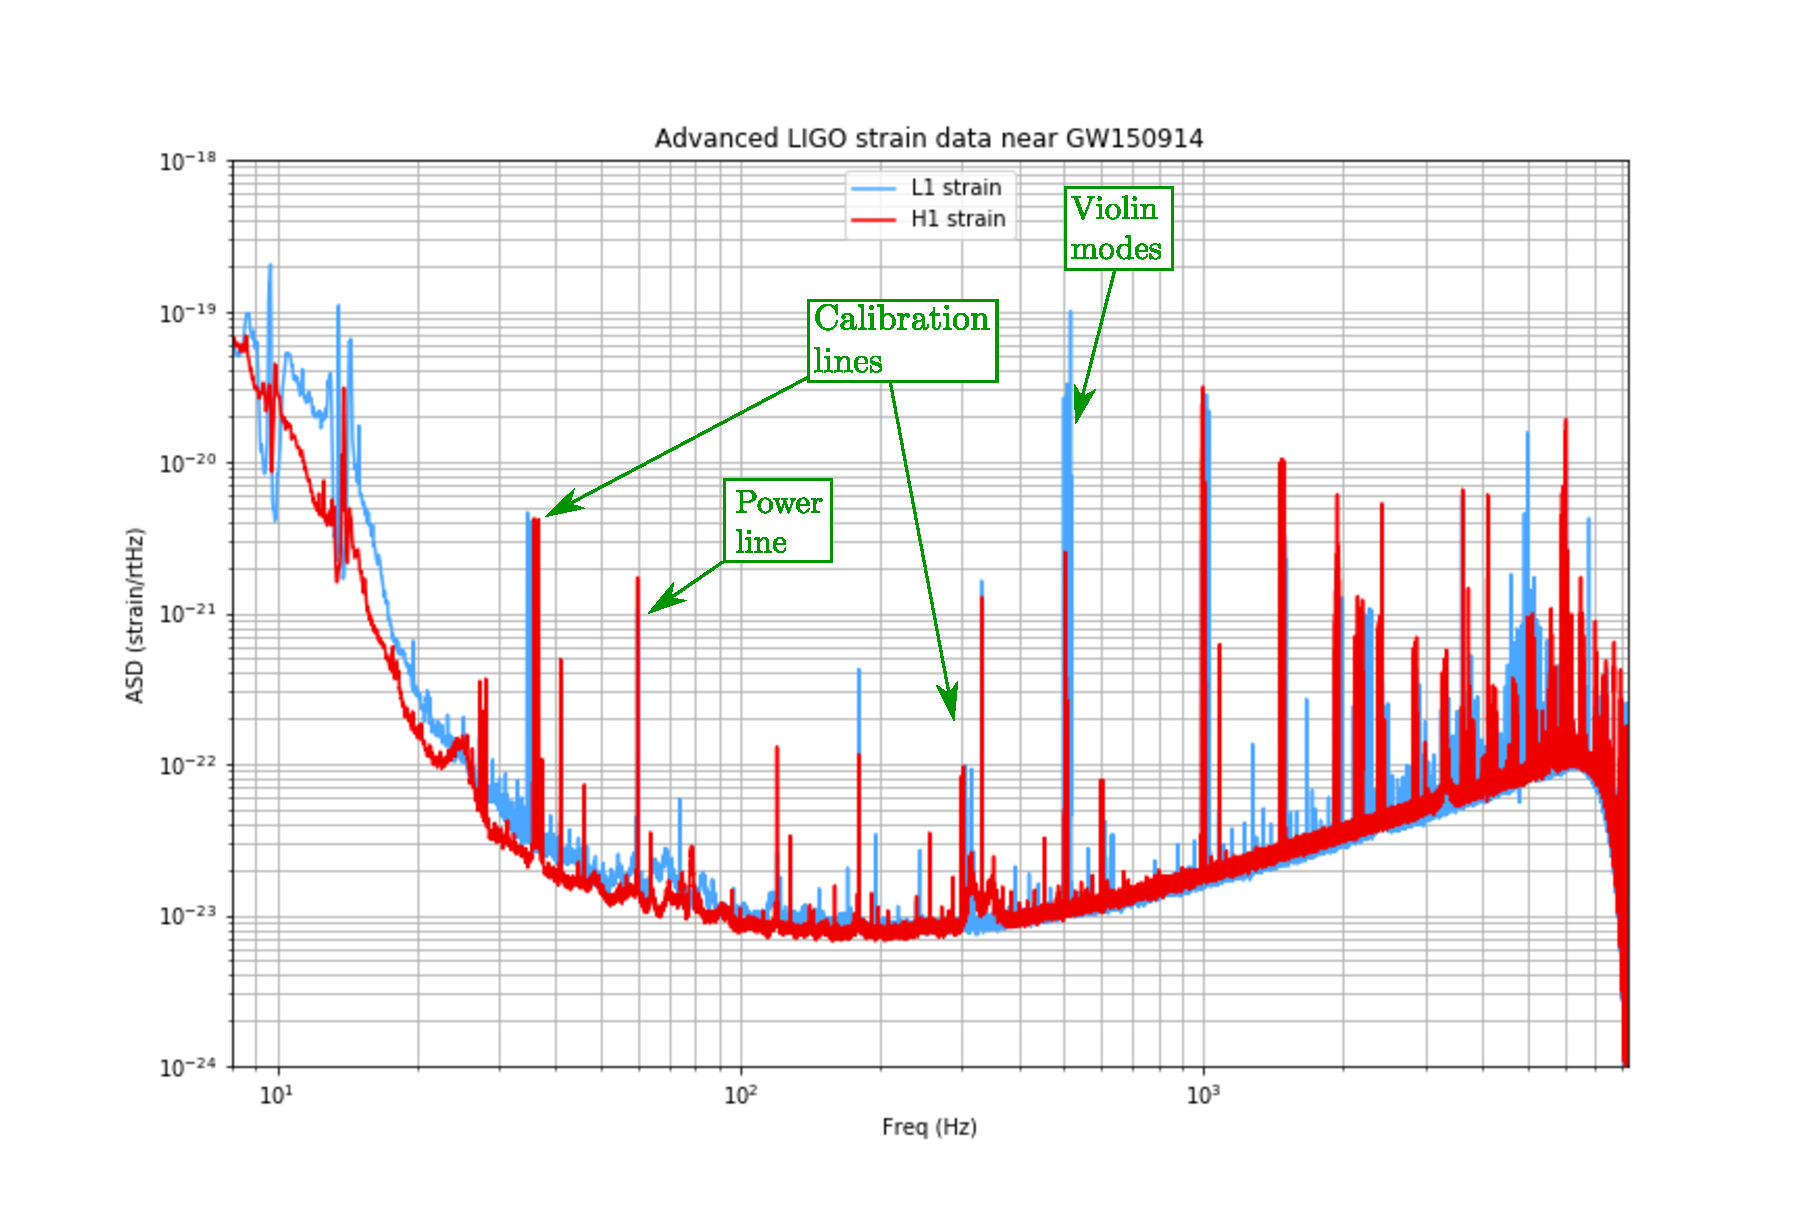
\includegraphics[width=\textwidth]{C6_detchar/ligo_o1_asd_annot.pdf}
\caption[Strain \gls{ASD} for the \gls{LIGO} detectors.]{
	The \gls{LIGO} detectors averaged \gls{ASD} is shown around the GW150914 event in O1 \citep{abbott2016ObservationGravitational}.
	This figure is from \citep{GWOpen} where the Power lines, Calibration lines and Violin modes are annotated. The
	power line from the mains in the USA is at 60 Hz. Some of the calibration lines
	are around 30 Hz, 331 Hz and 1083 Hz. The various violin modes of the suspensions are at 300, 500, 600 and 900 Hz where I have only marked the 500 Hz mirror suspension modes \citep{GWOpen}.} 
	\label{detchar:line:psd} 
\end{figure}
%
The \gls{ASD} in Fig.~\ref{detchar:line:psd} shows the time averaged spectra
of the \gls{GW} channel of the \gls{LIGO} detectors. The lines seen in the spectrum are not from any \gls{GW}
and are usually from terrestrial sources.  To see the lines in the \gls{GW}
channel, they must be transferred via some mechanism to this channel, known as coupling in.  There are a number of
ways in which this happens which are outlined in
\citep{covas2018IdentificationMitigation}.  This includes coupling via shared
power sources and shared grounds or earth's in the electrical circuits.  When different components share the same power supplies, if
a component draws power with a given period, then the voltage will decrease
repeatedly at this frequency.  Another component which shares this same power
supply can then also see this drop in voltage and this can potentially become
visible in a recorded output.  Another mechanism is coupling through magnetic
fields, this is common when cables are close to each other, the magnetic field
in one can affect the other, therefore, coupling noise between different
systems.  Coupling can also occur though a physical connection, known as
mechanical coupling, for example the resonances of the suspension fibers which
couple directly into the mirrors and therefore the output error signal.

%
% Origins of some lines and how they can be mitigated

Many of the spectral lines seen in the frequency spectrum in
Fig.~\ref{detchar:line:psd} are fundamental to the design of the detector.
These are difficult to eliminate at their source, therefore need to be understood such that their
effect on searches is minimised.  Some of the strongest of these lines are
listed below:

\begin{description}
	\item[Power line] The power line harmonics are fundamental to the
	detector and originate from the mains power supply in the
	\gls{USA}. These lines exist at 60 Hz which is the frequency of the
	mains alternating current \citep{aasi2015CharacterizationLIGO}. The European
	detectors Virgo and GEO have a power line at 50 Hz instead of 60 Hz.
	
    \item[Violin modes] The violin modes are associated with the
	suspensions fibers of the mirrors and the beam splitter in the detector. These are
	designed to have a narrow frequency spectrum such that they contaminate as
	small a part of the spectrum as possible. These are the lines around 500 Hz for
	the mirrors and 300, 600 and 900 Hz for the beam-splitter \citep{GWOpen} in
	Fig.~\ref{detchar:line:psd}.
	
	\item[Calibration lines] As described in Sec.~\ref{intro:detector} a \gls{GW} passing the detector will cause a change in the arm lengths of the interferometer, causing a power fluctuation at the output of the detector. 
	For stable operation of the interferometer, the power fluctuations are suppressed by using a feedback loop to control the detectors differential arm length. The error signal of this loop is then $h(t)$ \citep{ligoscientificcollaboration2017CalibrationAdvanced}.
	However, this is not entirely true as the transfer function of this feedback loop will affect the measurement of $h(t)$.
	It is therefore important to understand and correct for this feedback loop.
	The primary method for calibrating this is known as a photon calibrator \citep{karki2016AdvancedLIGO}.
	This applies a power modulated laser to the test mass, where the periodic force from radiation pressure appears as a calibration line in the detectors spectrum.
	This is then applied at a range of frequencies from a few Hz to several kHz \citep{karki2016AdvancedLIGO}.
	This can then be used along with other methods to calibrate the feedback loop \citep{ligoscientificcollaboration2017CalibrationAdvanced,coughlin2010NoiseLine,tuyenbayev2016ImprovingLIGO}.
 
\end{description}

Together with the fundamental lines of the detector, which are difficult to remove at the source, there are a large number of other lines whose source has been found and can be removed.  
Many of these are from mechanisms described
earlier such as shared power supplies or grounds. These can be removed by, for
example, using a different power supply for different systems. See
\citep{covas2018IdentificationMitigation} for a full investigation into the
mitigation of these lines.

%
% How lines affect CW searches

Instrumental lines have a large effect on all searches for \glspl{CW}, the lines can cause outliers in a search or can hide the \glspl{CW} power if the frequencies overlap or are close to the astrophysical frequency.
Searches for long duration \glspl{CW} are particularity sensitive to this type of artefact.  As described in
Sec.~\ref{searchcw}, \glspl{CW} are long duration signals with a slowly varying
frequency.  In the case of an isolated neutron star, the signal which is
searched for is a narrow-band sinusoid with a slowly varying frequency, where the frequency can be Doppler modulated by
the earth's rotation and orbit, and the amplitude is modulated by the antenna pattern of the detector as the earth rotates. For certain areas of parameter space, such as a sky position
close to the poles of the earth's orbit, the astrophysical signal of an isolated neutron star can
appear very similar to a narrow band fixed frequency instrumental line. The affect of many of these lines can be mitigated by using multiple detectors data. If a signal
appears in one detector and not the others, then it is likely that the signal
is from an instrumental line and not an astrophysical source.  These
contaminated frequency bands can either be removed or a statistic similar to
that described in Sec.~\ref{soap:las} or \citep{keitel2014SearchContinuous} can
be used to limit their effect.  However, there are many examples of
instrumental lines which appear at the same or similar frequencies in multiple
detectors.  These pose a real challenge to some \gls{CW} searches, and require
a substantial investigation to limit their affect.

%%%%%%%%%%
%%%%%%%%%%
\section{\label{detchar:monitor}Identifying and monitoring instrumental lines}
%%%%%%%%%%
%%%%%%%%%%
%
% into to why lines are monitored

When a detector is running, it is very important to identify instrumental lines
and monitor them.  The source of the line can potentially be located and its cause mitigated, or the line can be flagged such that astrophysical searches can avoid outliers near that frequency.  
The astrophysical searches use data from the \gls{GW} channel, therefore, the aim is to limit the affect of instrumental lines in this channel.

%
% Auxiliary channels 
In addition to the \gls{GW} channel, the detector
records many others known as auxiliary channels.  These channels
monitor many components of the detector, and importantly are not sensitive to
\glspl{GW}.  Many of the channels useful for line searches are the outputs of \glspl{PEM}.
\glspl{PEM} include sensors such as seismometers, temperature sensors,
magnetometers etc.  These channels can be very useful in identifying the source
of an instrumental line.  The main goal is to reduce the number of artefacts in
the \gls{GW} such that it is as close to Gaussian noise as possible.  If an
artefact shows up in the \gls{GW} channel in coincidence with one of the
\gls{PEM} then this is an indicator that the artefact originates from something
related to that \gls{PEM}.  For example, consider
that a magnetometer identifies a periodically changing magnetic field in a rack of electronics (which contains oscillators, clocks etc). If this a signal of the same frequency is observed the main \gls{GW} channel, this indicates that noise from this piece of electronics is somehow coupling into the detector.  One can then investigate the electronics near that magnetometer further to identify how and if it couples in.

%
% tools to monitor all the channels

There are a number of tools which teams of scientists use to monitor these spectral lines.
A summary of the results from these investigations for the first two observing runs of \gls{LIGO} can be found in
\citep{covas2018IdentificationMitigation}.  Some of the tools used to monitor these lines are
described below.

\begin{description}
	\item[Fscan] \Glspl{FFT} are taken of the raw detector data, typically these are 1800s long, for all of the auxiliary channels as well as the \gls{GW} channel.
	The power in each \gls{FFT} frequency bin is then normalised to a running median and then averaged over the set of \glspl{FFT} \citep{coughlin2010NoiseLine}.  After known lines such as Violin modes and power lines are
	subtracted, noise lines can be identified. A threshold can be set where spectrogram powers which exceed this threshold are flagged as a line. These
	can then be compared across multiple different channels. More detail on how the
	lines are identified can be found in \citep{coughlin2010NoiseLine}.
	
    \item[Coherence] This tool searches for the coherence between different
	channels and different detectors. This is similar to searches for the stochastic
	gravitational wave background \citep{allen1999DetectingStochastic}. This uses the cross correlation between two different channels, this can be different detectors \gls{GW} channels or a \gls{GW} channel and a \gls{PEM} channel. 
	Significant lines are then found by setting thresholds on the values of the coherence, where these can be flagged for further investigation.
	More detail of how this works can be found in \citep{covas2018IdentificationMitigation,coughlin2010NoiseLine,}.
	
	\item[Finetooth] If a line exhibits some periodic amplitude or frequency modulation, then it can appear as harmonics in the frequency spectrum, where the collection of regularly spaced harmonics make up a `comb'. 
	Many of the instrumental lines identified in the spectrum are then not from separate sources but are part of `combs' which originate from a single source. 
	These combs are characterised by their start frequency and the spacing of the harmonics (tooth spacing).
	Finetooth is a tool which identifies and monitors these combs \citep{neunzertDailyComb}.
	\joe{say what this actually does}

	
	\item[\Gls{NoEMi}] This tool uses various methods to identify peaks in an \gls{SFT}, analyse these peaks, find coincidences between \glspl{SFT} and tracks lines. 
	The method initially runs a peak finding algorithm on each \gls{SFT}, and for each peak stores the frequency, width, amplitude and \gls{CR}, which is defined as the difference between the peak amplitude and the mean value of the spectrum divided by the spectrum's standard deviation.
	These peaks are then analysed by investigating the peaks found in $\mathcal{O}(10)$ \glspl{SFT}. 
	The distribution of the peaks in frequency can be used to identify stationary instrumental lines. 
	Looking at the \gls{CR} versus frequency, can help identify non-stationary lines.
	Coincidences can then be found by comparing the peaks identified in the \gls{GW} channel and some auxiliary channel. 
	The time evolution of the line is then reconstructed such that it can be tracked.
	Each of the identified lines is then stored in a database.
	More details on this pipeline can be found in \citep{accadia2012NoEMiNoise}.

	
\end{description}


These tools offer different methods to identify and mitigate instrumental lines, and more generally understand the noise of the detector. A summary of these efforts for
the advanced \gls{LIGO} data can be found in
\citep{covas2018IdentificationMitigation}, or specifically for O3 on the \gls{LIGO} wiki page {\tt
\url{https://wiki.ligo.org/DetChar/O3LinesCombsInvestigations}}. The following
sections describe how the SOAP search described in chapter \ref{soap} can be used
as an extra tool to aid in the identification and monitoring of instrumental
lines.


%%%%%%%%%%%
%%%%%%%%%%%
\section{\label{detchar:soap}Identifying instrumental lines with SOAP}
%%%%%%%%%%%
%%%%%%%%%%%%

% Why SOAP may be good at finding instrumental lines
% 
The SOAP search has been tested on a number of observing runs
to search for \gls{CW}.  One of the major factors that limited the sensitivity
of the search, is the presence of instrumental lines within the data.  Many of
the potential candidates which SOAP returned could be identified as an
instrumental line.
%
\begin{figure}[hp]
	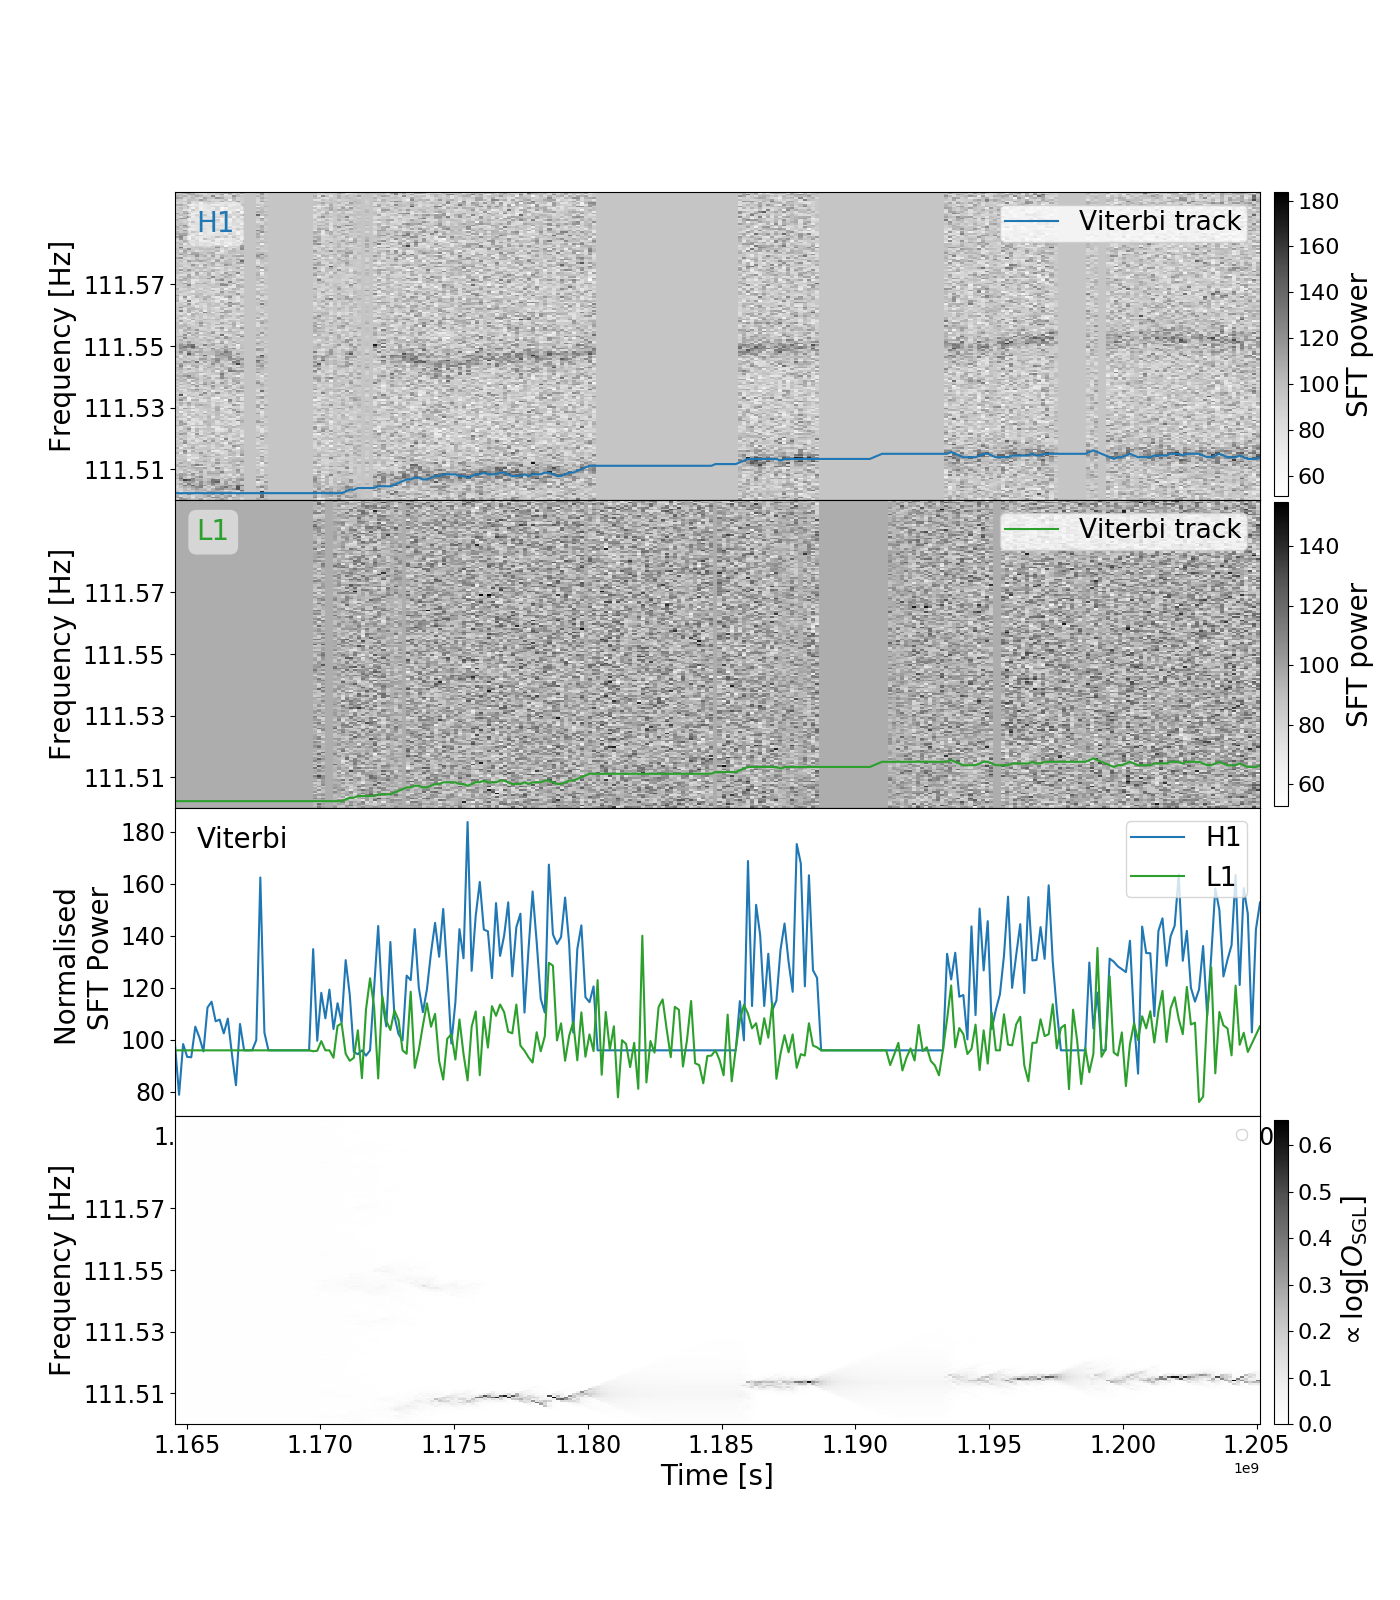
\includegraphics[width=\textwidth]{C6_detchar/plot_F111_5_wandering_line.png}
        \caption[Broad wandering line example.]{ The spectrograms generated from 1800s long \gls{SFT} which are summed over one day are shown for H1 and L1 in the top two panels, where two broad wandering lines can be seen in H1.
        The Viterbi track returned by the SOAP astrophysical search described in chapter \ref{soap} is overlaid on each of these spectrograms.
        The third panel shows the normalised spectrogram power along the Viterbi track for each of the detectors. The final
        panel shows the Viterbi map for this frequency band.
			}
\label{detchar:soap:astrowander}

\end{figure}
%
Figure \ref{detchar:soap:astrowander} shows a broad and wandering line during the O2 observing run, where the line in H1 is causing the SOAP search to mistake the track for an astrophysical signal.
This is because the SOAP line-aware statistic from Sec.~\ref{soap:las} finds
areas of higher power which are consistent between detectors. These types of line are difficult to mitigate in an astrophysical
search as there is consistent high \gls{SFT} power in both the broad line and the noise in the other detector.
However, this has a side effect of being useful to identify the
instrumental lines themselves.
In this section, I will explain the setup of the SOAP search to identify
instrumental lines.

It is often useful to search through the auxiliary channels when trying to
identify the source or a line. 
This would involve using the multiple detector search described in Sec.~\ref{soap:multidet} to identify lines which are coincident between channels. 
The aim of this section however, is to flag potential lines within the \gls{GW} channel in individual detectors.
Whilst we have developed a statistic in Eq.~\ref{soap:las:stat} to penalise line like signals, we revert to using the
`normalised' \gls{SFT} power as the statistic in the SOAP search. The single
detector search then has one parameter to vary, the transition matrix
parameter $\tau$.  This governs how probable the frequency track is to transition up,
straight or down a frequency bin.  In this search we are aiming to find any line-like artefact.
Therefore, we allow an equal probability for the track to jump in any
direction, but limit it to change by one frequency bin after each time
segment.  

In the astrophysical search, the \glspl{SFT} were summed over one day to take the average over the antenna pattern such that the \gls{SNR} in each detector is similar and to increase the \gls{SNR} in a given frequency bin.
However, in the line search, there is not antenna pattern to average over and the majority of instrumental lines are expected to have a higher \gls{SNR} than astrophysical signals.
Therefore the search is run over normalised 1800s long \glspl{SFT}, which also reduces the preprocessing time of the search.
The 1800s \glspl{SFT} are also generated as part of the Fscan search described in Sec.~\ref{detchar:monitor}, therefore, this reduces the computational cost of generating \glspl{SFT} as part of this search. 
For this line search, we split the 1800 s \glspl{SFT} into 0.1 Hz wide sub-bands and run the single detector search on each sub-band. 
The search then returns the same outputs as described in
Sec.~\ref{soap} and Sec.~\ref{machine}: the frequency track (Viterbi track), a
Viterbi map and a Viterbi statistic.  Here the Viterbi statistic is just the
sum of the \gls{SFT} power along the frequency track.  

These three outputs can then indicate whether an instrumental line is present within any given sub-band.
Initially, one can look at the distribution of the Viterbi statistics for each sub-band, Fig.~\ref{detchar:soap:rankedstats} shows a histogram of the Viterbi statistics from the H1 detector between 40-500 Hz for the O3 observing run.
%
\begin{figure}[ht]
	\centering
	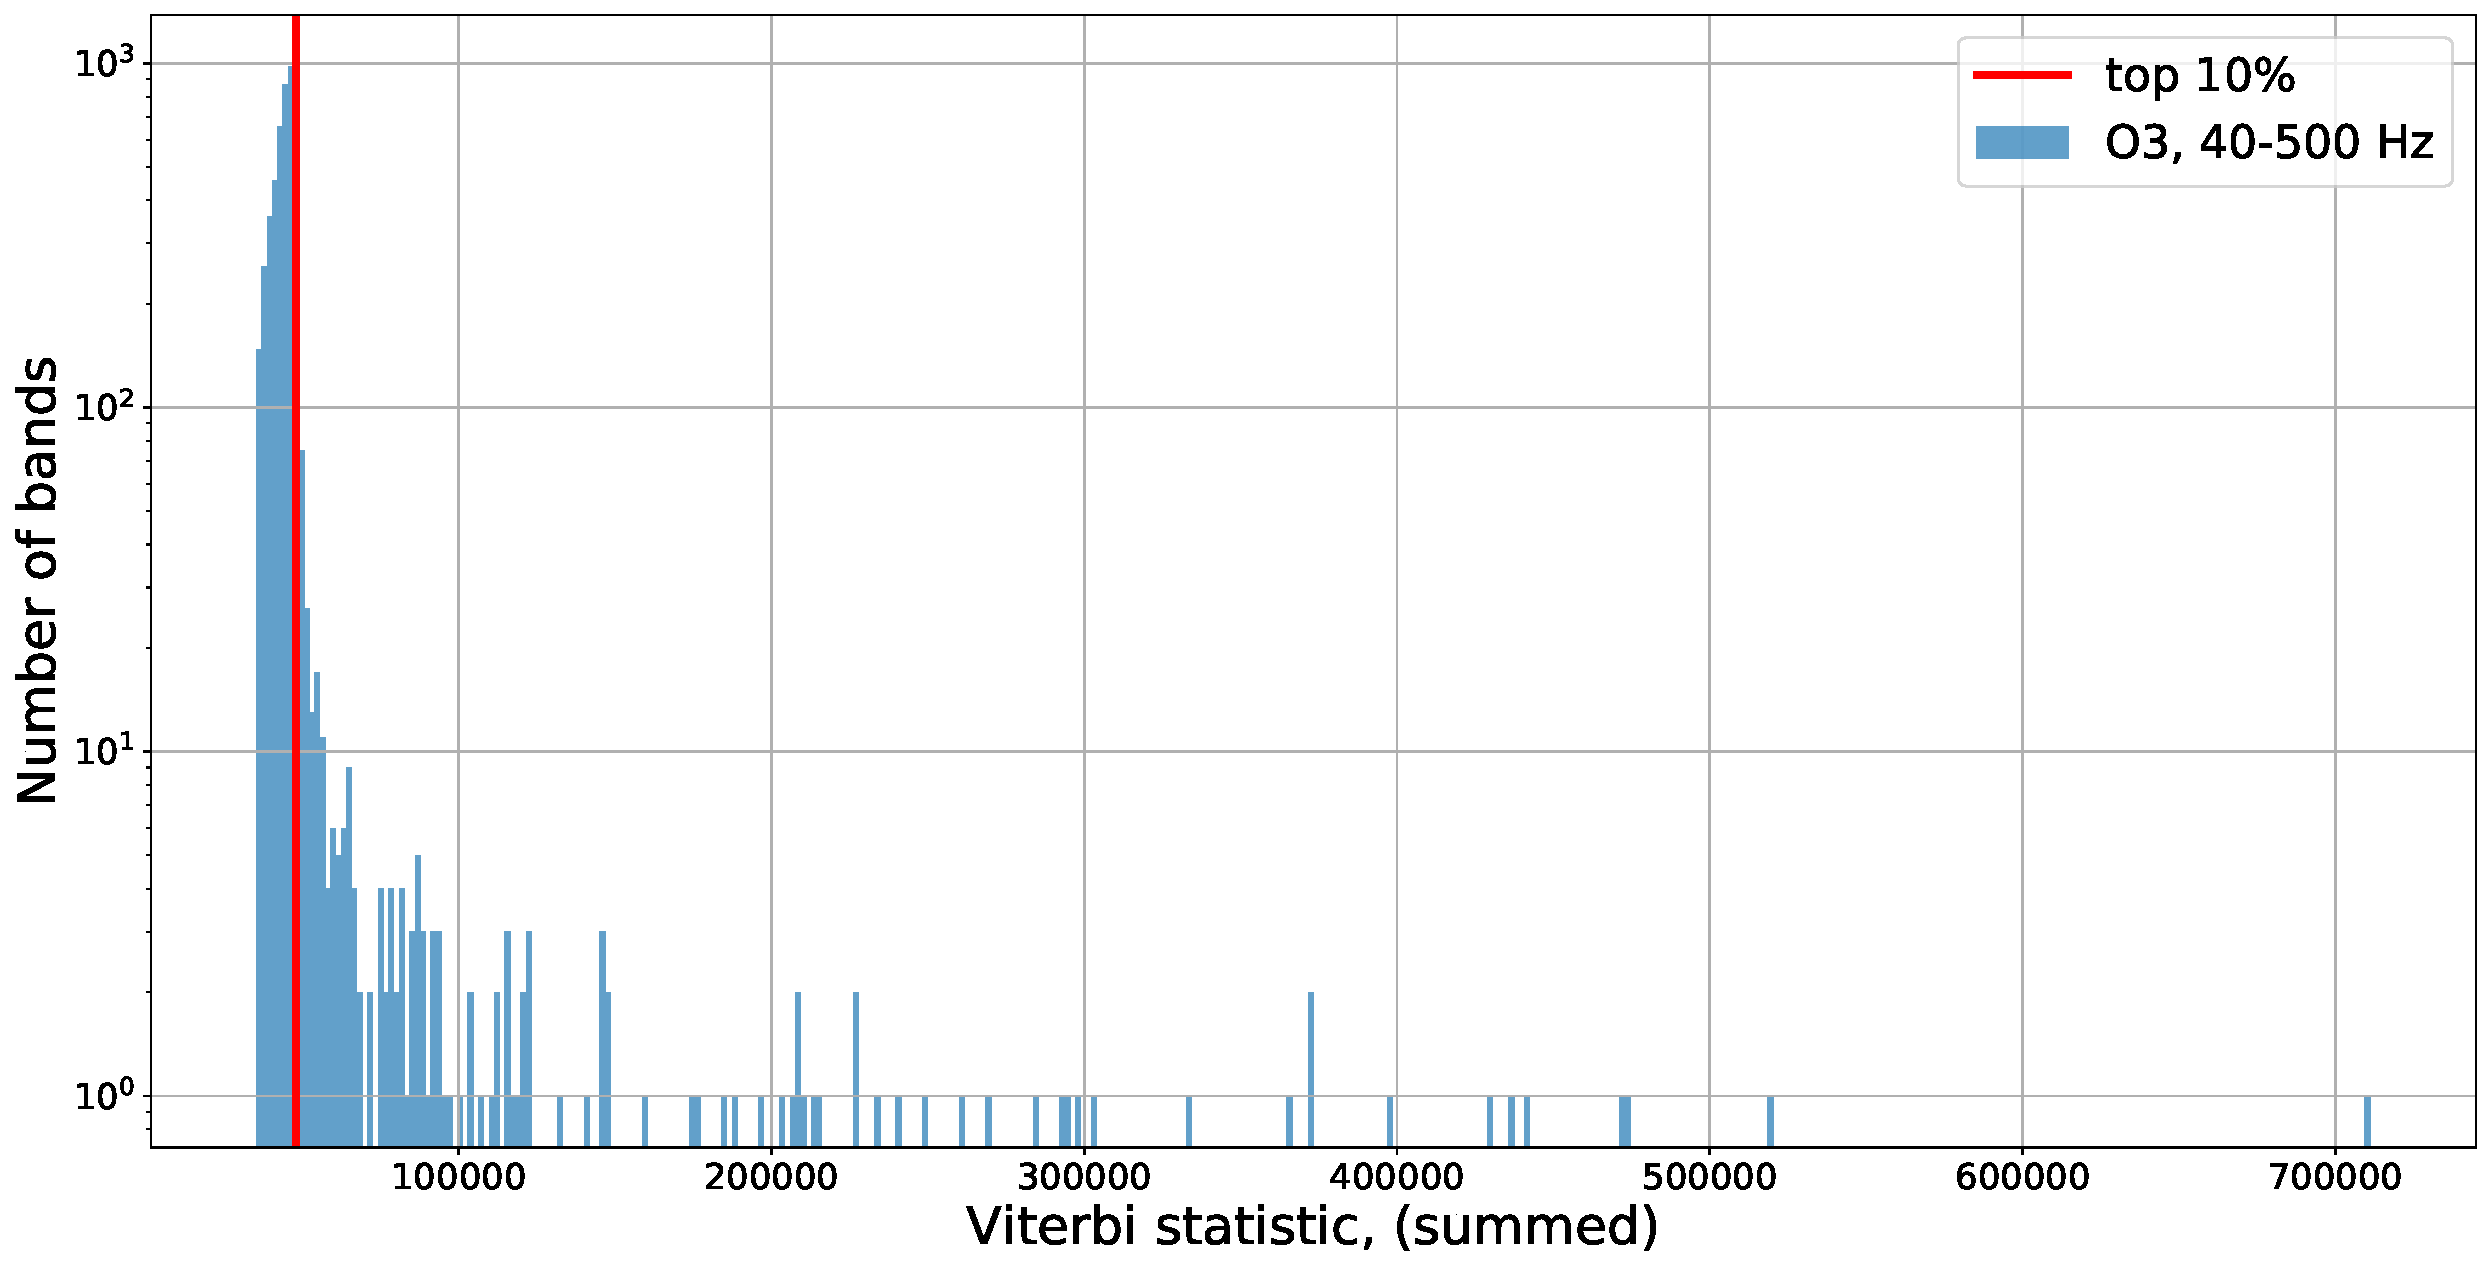
\includegraphics[width=\textwidth]{C6_detchar/statistic_hists_O3_H1.pdf}
	\caption[Viterbi statistics for H1 in O3, 40-500 Hz]{This shows a histogram of the Viterbi statistics from the SOAP search from chapter \ref{soap}, where the statistic is the summed \gls{SFT}  power along the Viterbi track. These results are between 40-500 Hz for the Hanford detector (H1) during the O3 observing run. The red line indicated where 10\% of the Viterbi statistics are larger than this value. }
	\label{detchar:soap:rankedstats}
\end{figure}
%
This shows that the majority of sub-bands fall within a single distribution, where larger values of the Viterbi statistic are good indicators that there is an instrumental line present within the sub-band.
One can the define a list of potential instrumental lines by taking the top 10\% of Viterbi statistics. 
These can then be investigated further by looking into other outputs of the SOAP search, including the Viterbi map and the Viterbi track.

%
% Introduce the plots
The line search then outputs plots as shown in Fig.~\ref{detchar:soap:noiseplot}, \ref{detchar:soap:lineplot} and
\ref{detchar:soap:wanderplot}. 
There are three panels to each plot: the first shows the the normalised \gls{SFT} power searched through by SOAP with the Viterbi track overlaid and the second panel shows the output Viterbi map.
The final panel shows the \gls{SFT} power along the Viterbi track and the mean noise floor of the detector as a function of time in the frequency band.  
The aim is to use the information contained within these plots and the equivalent ones for other sub-bands to classify each sub-band into containing an instrumental artefact or not. 

%
% Features in the noise plot
There are certain features in each of the panels in, for example, Fig.~\ref{detchar:soap:noiseplot} which indicate that SOAP has identified a potential line within a sub-band or not.
The Viterbi track in Fig.~\ref{detchar:soap:noiseplot} appears to be randomly wandering around the full width of the sub-band, implying that there is no strong signal within the band which SOAP can identify.
The Viterbi statistic also falls in the main distribution of statistics in Fig.~\ref{detchar:soap:rankedstats}, whilst this would not show up in the to 10\% of Viterbi statistics, I describe it here to show the differences in the outputs compared to when there is a line.
The second panel of Fig.~\ref{detchar:soap:noiseplot} which shows the Viterbi map, contains no areas of high log probability and no clear long duration features. These features will become apparent in Fig.~\ref{detchar:soap:lineplot} and \ref{detchar:soap:wanderplot}.
The normalised \gls{SFT} power along the Viterbi track shows values which are consistent with a $\chi^2$ distribution with two degrees of freedom, which has a mean of two, implying that the \gls{SFT} power along the track follows the expected noise distribution.
Each of these indicate that there is no line present within this sub-band.
%
\begin{figure}[hpt]
	\centering
	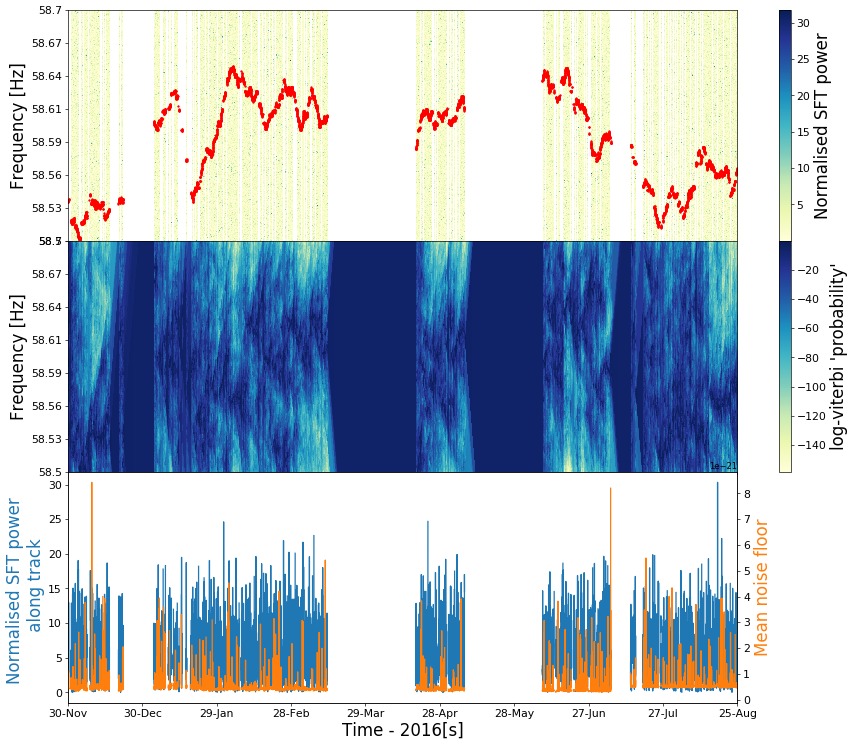
\includegraphics[width=\textwidth]{C6_detchar/track_F58_5_58_7_noise.png}
	\caption[Example SOAP output for Gaussian like noise.]{The SOAP search outputs three main
quantities, the Viterbi maps, the Viterbi track and the Viterbi statistic. The
Viterbi track is shown above overlaid onto the 1800s \gls{SFT} power spectrum
including the detector gaps for \glspl{LIGO} Hanford detector (H1) in its
third observing run (O3). This track is an indicator as to what the SOAP search has identified within the band, where this track indicates that SOAP has identified noise and no signal. The returned Viterbi statistic is also consistent with that of noise.
The Viterbi map is another visualisation of the sub-band, how to interpret this
has been explained in chapters \ref{soap} and \ref{machine}. The final panel is a way to visualise how the \gls{SFT}
power changes along the Viterbi track. Also on this plot is an estimate of the
mean noise floor for this band to visualise how the sensitivity of the detector
changed over the course of the run.}

	\label{detchar:soap:noiseplot}
\end{figure}

%
% Features in the narrow line plot

If we then look at the outputs of Fig.~\ref{detchar:soap:lineplot}, we see a Viterbi track which is spread over a narrow frequency range ($\mathcal{O}(1)$ frequency bins) for the entire duration of the run.  
This indicates that there is areas of \gls{SFT} power around this frequency which is higher than other areas in the sub-band.
In the Viterbi map in the second panel of Fig.~\ref{detchar:soap:lineplot}, the log-Viterbi probability is contained within a narrow frequency range around the Viterbi track.
This again indicates that there is a narrow spectral line within this sub-band.
Finally the third panel shows the \gls{SFT} power along the Viterbi track, which no longer follows a $\chi^2$ distribution but had a large excess of power.
Each of these features are strong indicators that there is an instrumental line present within this sub-band.
%
\begin{figure}[hpt]
	\centering
	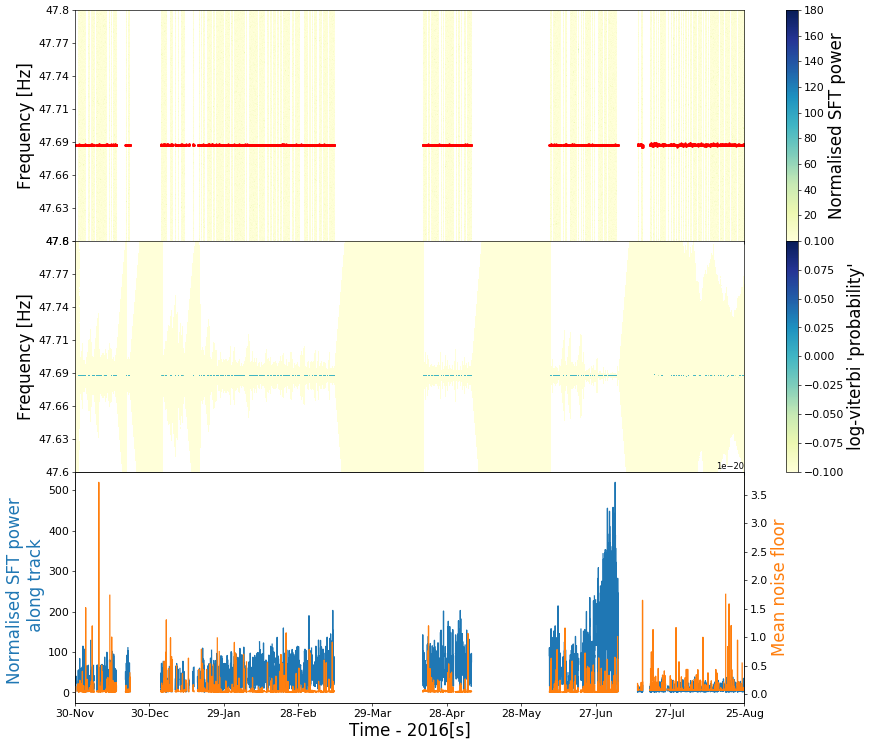
\includegraphics[width=\textwidth]{C6_detchar/track_F47_6_47_8_linenarrow.png}
	\caption[Example SOAP output for string narrow instrumental line.]{The equivalent plot as in Fig.~\ref{detchar:soap:noiseplot} can be made when there is a narrow spectral artefact in the band. The above is again results from \glspl{LIGO} Hanford detector (H1) in its third observing run (O3) using 1800s \gls{SFT} power spectrum. In this there is a narrow spectral line at $\sim 47.69$ Hz, where the Viterbi track follows this line of high power. The Viterbi map has much higher values for the log-probability in this line case compared to the noise case, this is an indicator some real signal. The probability in the Viterbi maps drops to zero in some areas due to the strength of the instrumental line, these are the white areas in the Viterbi map plot (second panel). }
	\label{detchar:soap:lineplot}
\end{figure}
%


%
\begin{figure}[hpt]
	\centering
	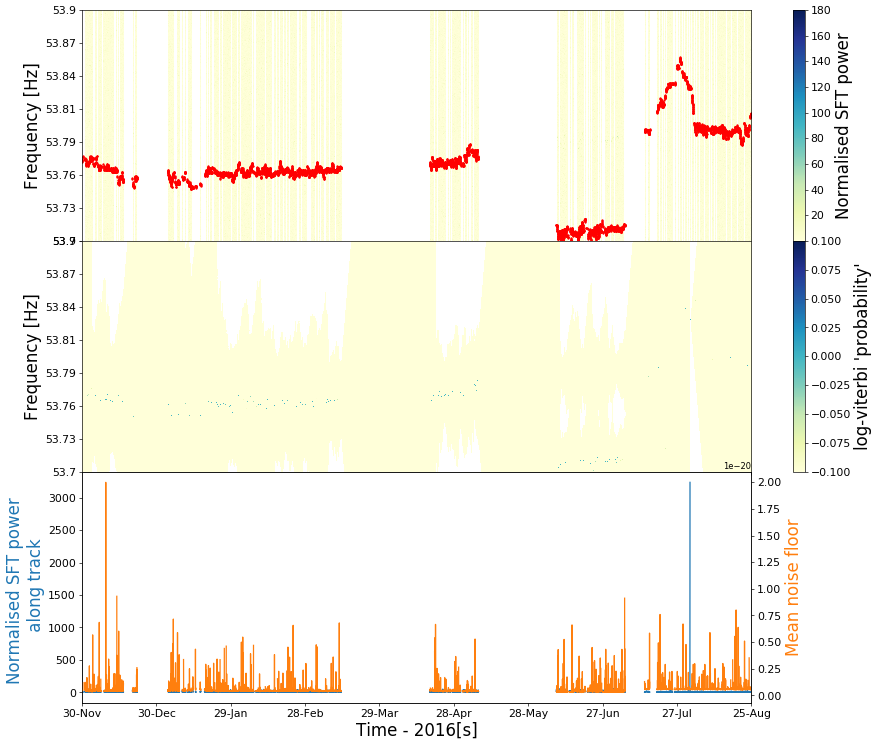
\includegraphics[width=\textwidth]{C6_detchar/track_F53_7_53_9_wander.png}
	\caption[Example SOAP output for wandering line.]{The equivalent plot as in Fig.~\ref{detchar:soap:noiseplot} can be made when there is a wandering spectral line. The above is again results from \glspl{LIGO} Hanford detector (H1) in its third observing run (O3) using 1800s \gls{SFT} power spectrum. This shows how some spectral lines do not have a fixed frequency and can wander through the band. These are especially hard to track and monitor. The Viterbi track here shows is clearly different from the noise case in Fig.~\ref{detchar:soap:noiseplot} as the track is more tightly concentrated around some areas of power. }
	\label{detchar:soap:wanderplot}
\end{figure}
%

Figure \ref{detchar:soap:wanderplot} shows the equivalent plots to
Fig.~\ref{detchar:soap:noiseplot} and \ref{detchar:soap:lineplot} but now
contains a wandering spectral artefact.  This is
a line which wanders in
frequency as is moves though time.  This can be seen in the frequency
track, which here does not have much spread, however, the frequency of the
track changes with time.  There are also areas where the track switched to a separate spectral artefact within the same
band.  SOAP only returns a single track which follows that of the highest \gls{SFT} power, if there are multiple spectral artefacts within a sub-band, then SOAP will identify the areas of high power in each which correspond to the highest sum of \gls{SFT} power.
This means that the track can, and does, switch between different spectral artefacts accumulating the highest \gls{SFT} power from each.
Fig.~\ref{detchar:soap:wanderplot} shows this discrete jump around
January.

\clearpage

The Viterbi statistic is used as an initial flag for a sub-band which could potentially contain an instrumental line.
The equivalent plots as in Fig.~\ref{detchar:soap:noiseplot}, \ref{detchar:soap:lineplot} and
\ref{detchar:soap:wanderplot} for each sub-band can then be used for further investigation, where this investigation can provide a list of potential lines. 
We generated a list of potential instrumental lines for \glspl{LIGO} third observing run (O3) between 40 and 500 Hz.
This line list can then be compared to existing O3 \gls{LIGO} line lists which are generated using the searches described in Sec.~\ref{detchar:monitor}.
There are currently two line lists produced by \gls{LIGO} scientists, one which contain lines where the source has been identified and one where the source is not known.
Known lines can be accessed at {\tt \url{https://ldas-jobs.ligo-wa.caltech.edu/~evan.goetz/CW/O3aLines/H1/index.html}}
and unknown lines at {\tt \url{https://ldas-jobs.ligo-wa.caltech.edu/~evan.goetz/CW/O3aLines/H1/Unidentified/index.html}} or are both stored in a git repository {\tt \url{https://git.ligo.org/CW/instrumental/aLIGO-lines-combs}}. 

These line lists can be compared to the list of lines generated by SOAP to compare its performance to existing techniques.
For the SOAP search we count the line as detected if the sub-band which contains the line has an associated Viterbi statistic which crosses the 10\% threshold from Fig.~\ref{detchar:soap:rankedstats}.
SOAP then detected 55\% of the lines of known origin and 30\% of the lines where the origin is not known.
Of the lines of known origin, all of those which SOAP did not identify were from ``Calibration line mixing'' or ``Calibration line non-linearity'' \joe{woudl be nice to have a reference, cant find much rn}, upon further investigation of these frequency bands, we found that these lines appear as short duration ($< 1$ week) signals in SOAP's output, where some examples of these can be seen in Fig.~\ref{detchar:soap:calibrationlinemixing}.
SOAP struggles to find short duration signals as is the signal is weak it cannot build up enough \gls{SNR} to pass the detection threshold, however, the line is still visible when investigating the Viterbi maps and Viterbi track. 
%
\begin{figure}[hpt]
	\centering
	\begin{subfigure}[h]{0.49\textwidth}
		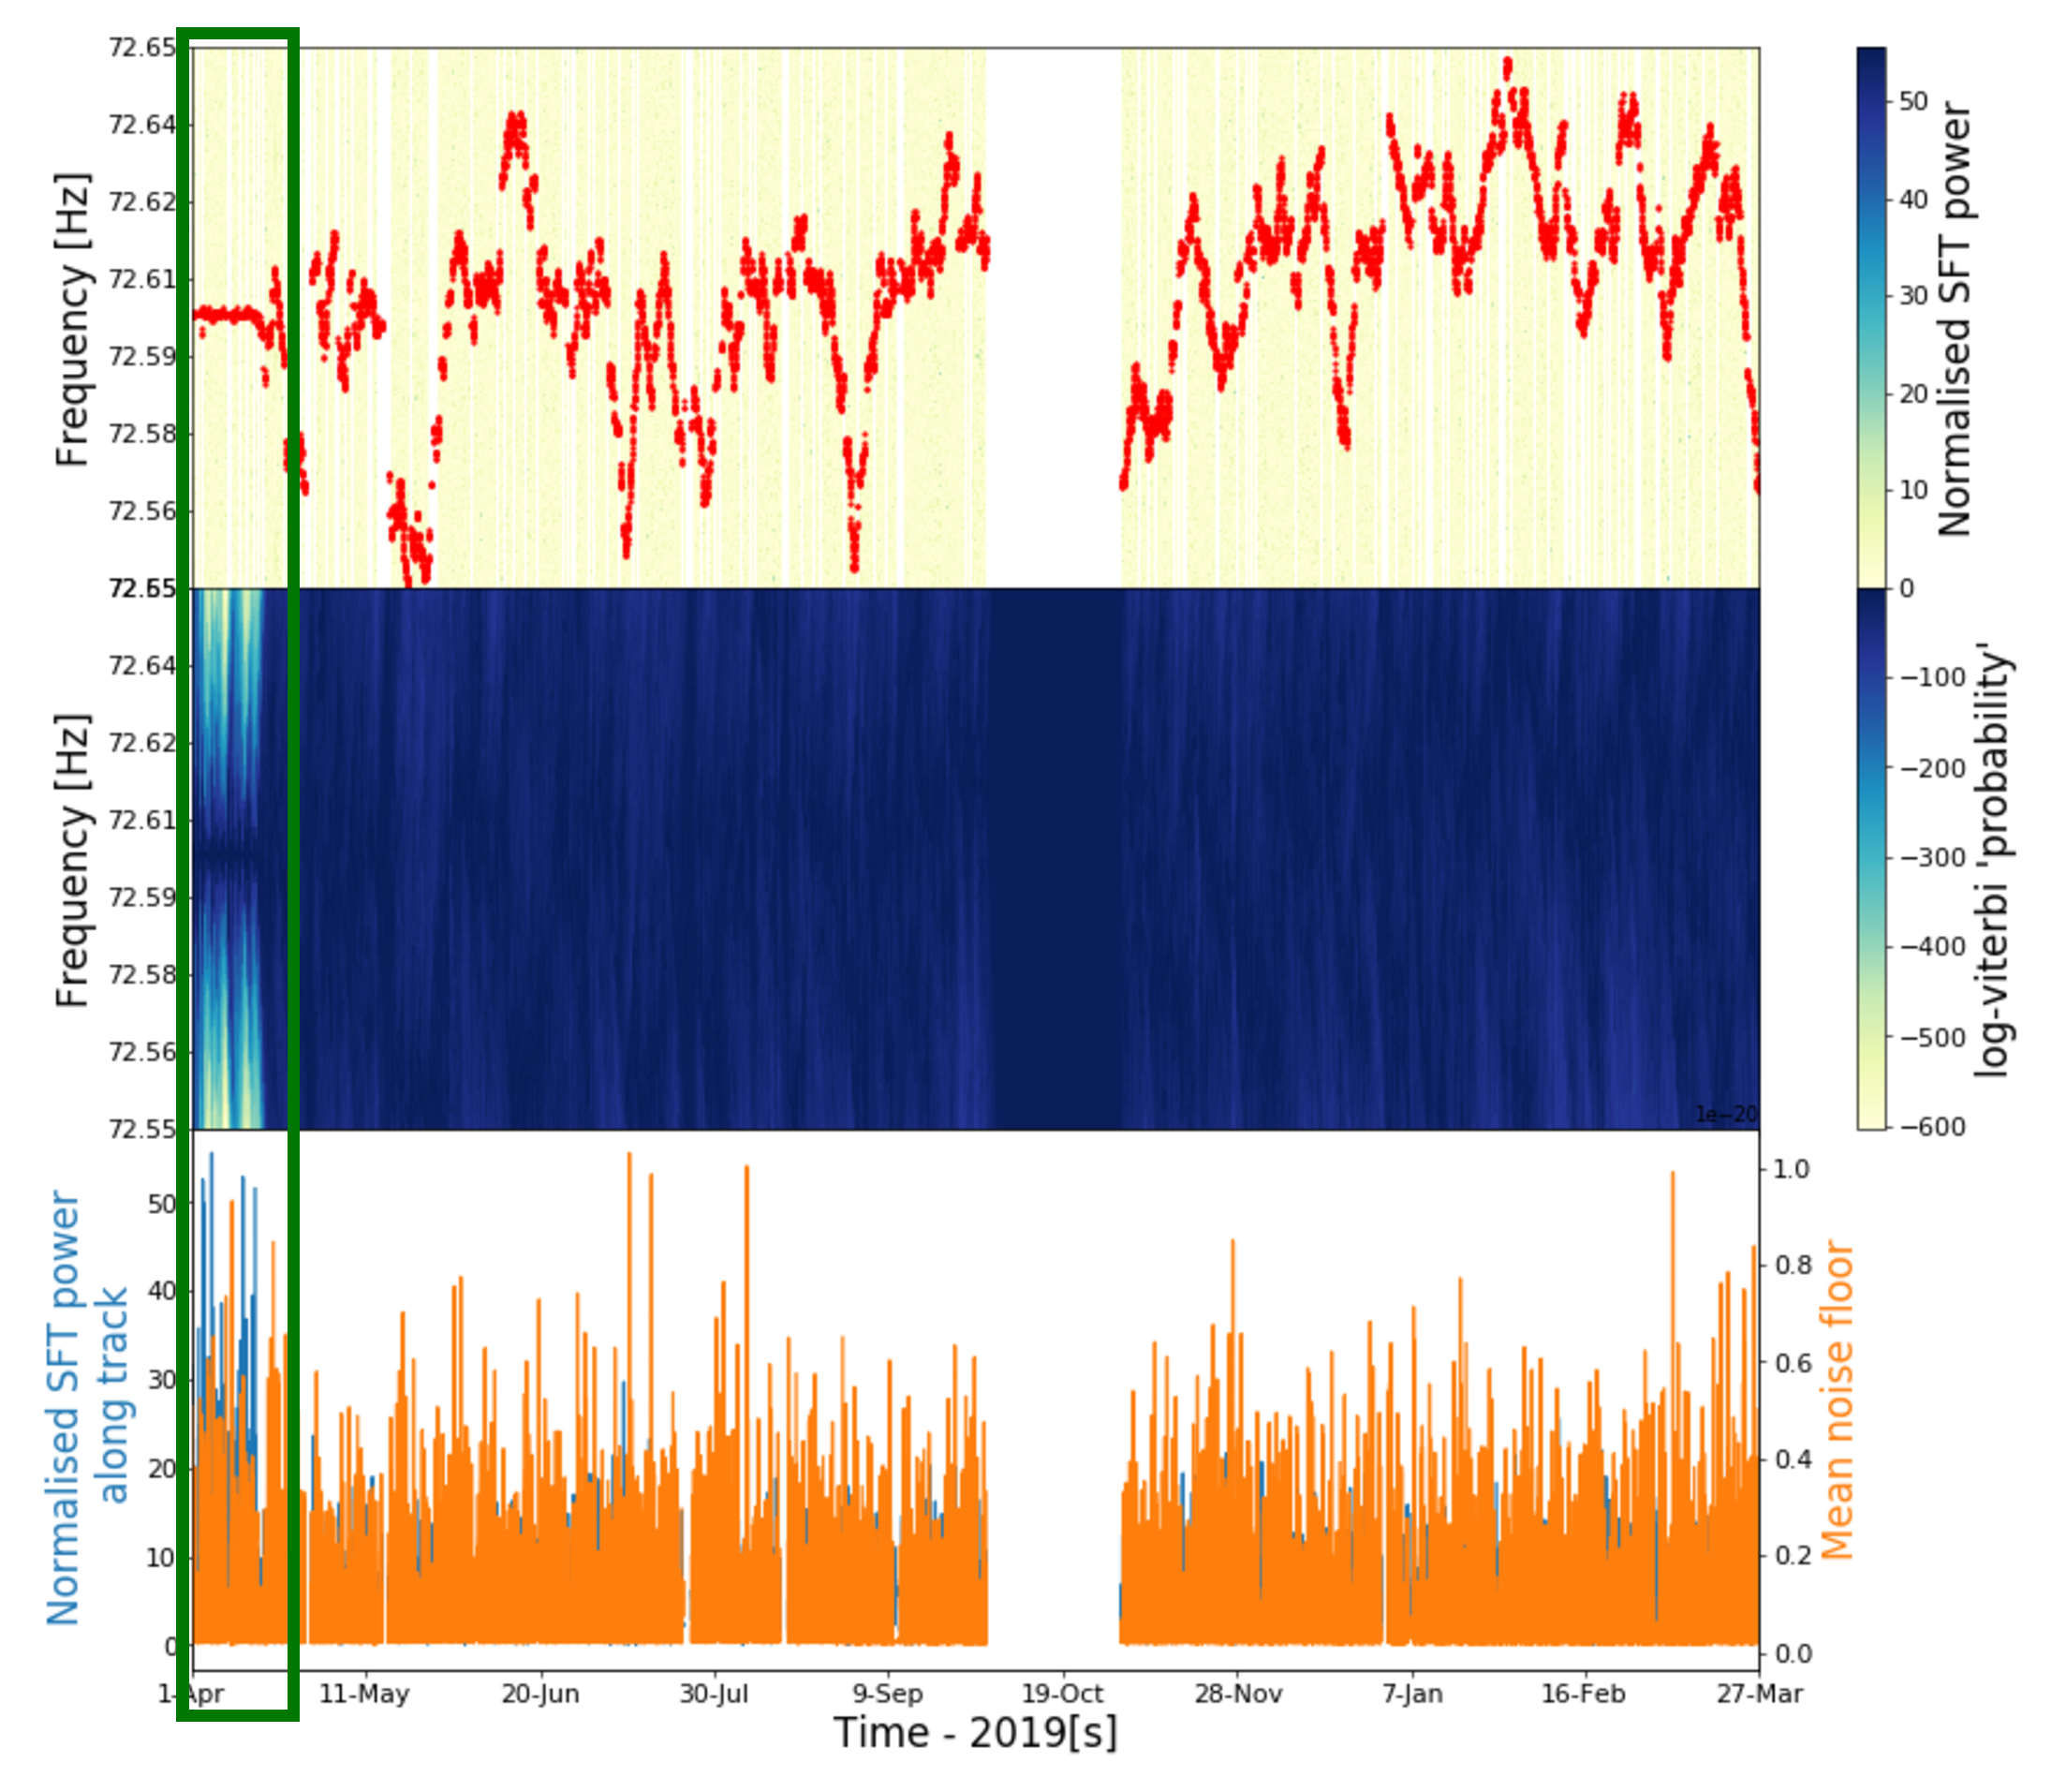
\includegraphics[width=\textwidth]{C6_detchar/linemixing/track_F72_55_72_65.pdf}
		\caption{\label{detchar:soap:calibrationlinemixing:1}}
	\end{subfigure}
\begin{subfigure}[h]{0.49\textwidth}
	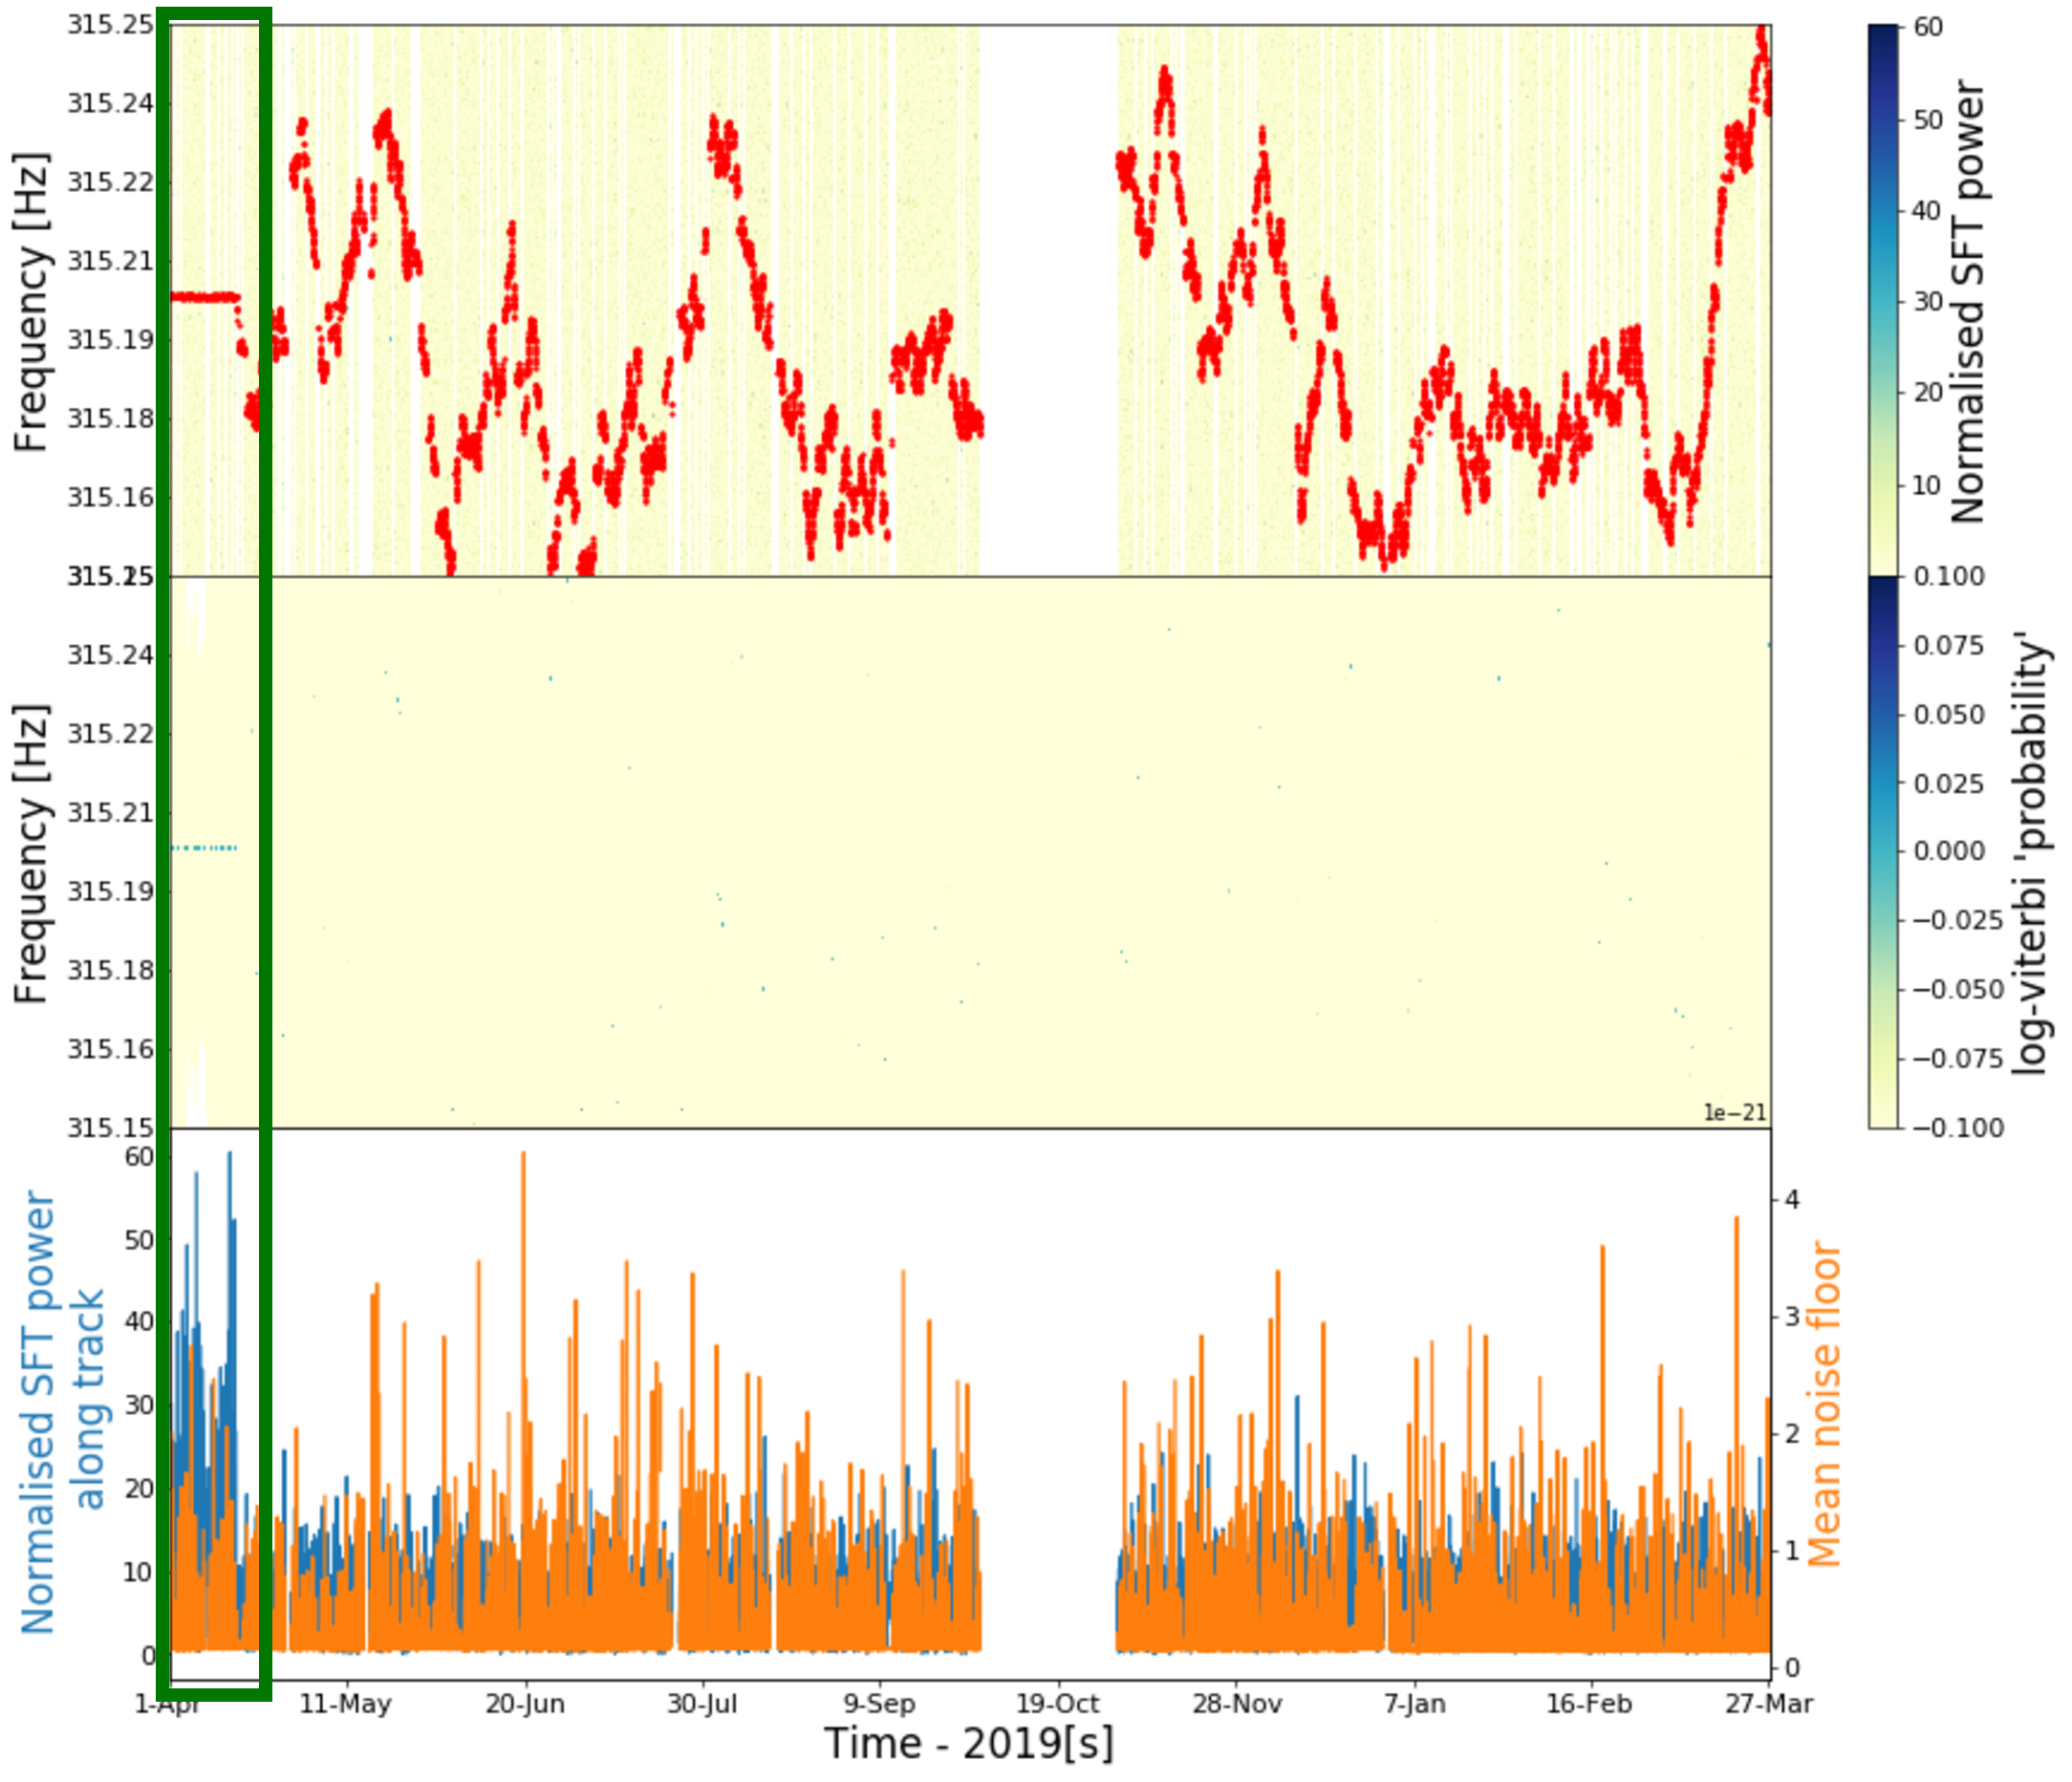
\includegraphics[width=\textwidth]{C6_detchar/linemixing/track_F315_15_315_25.pdf}
	\caption{\label{detchar:soap:calibrationlinemixing:2}}
\end{subfigure}

\begin{subfigure}[h]{0.49\textwidth}
	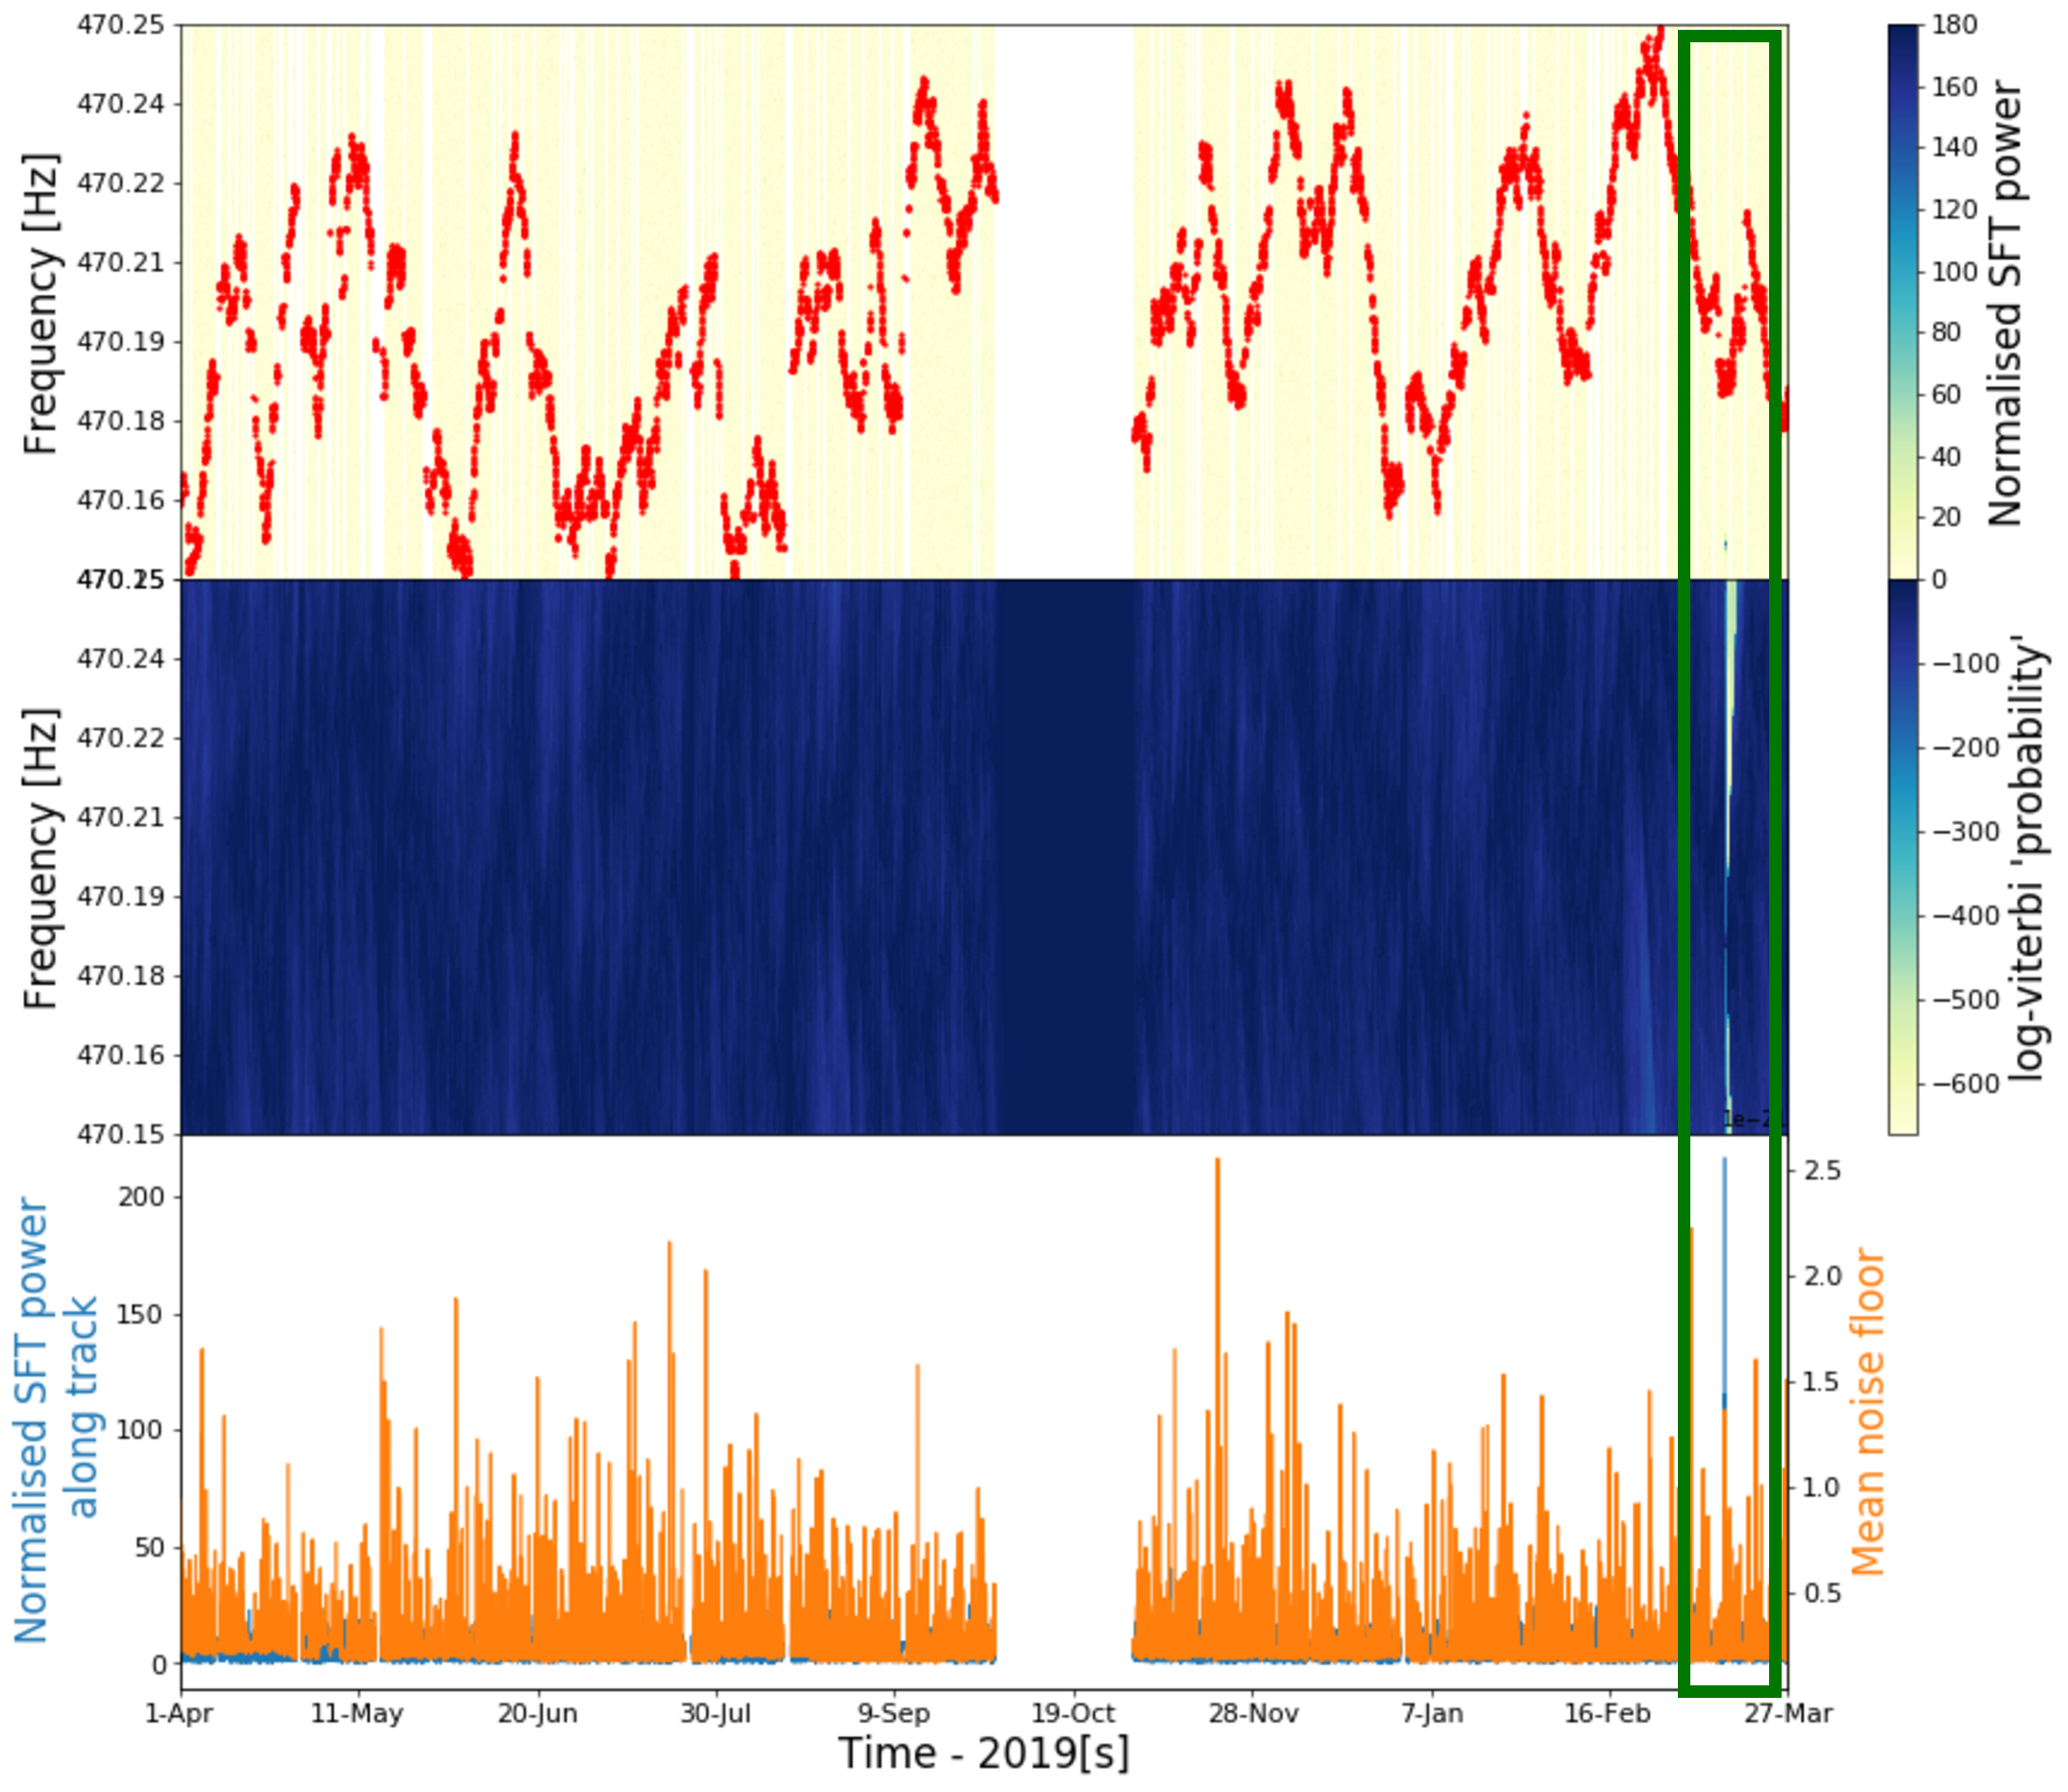
\includegraphics[width=\textwidth]{C6_detchar/linemixing/track_F470_15_470_25.pdf}
	\caption{\label{detchar:soap:calibrationlinemixing:3}}
\end{subfigure}
\begin{subfigure}[h]{0.49\textwidth}
	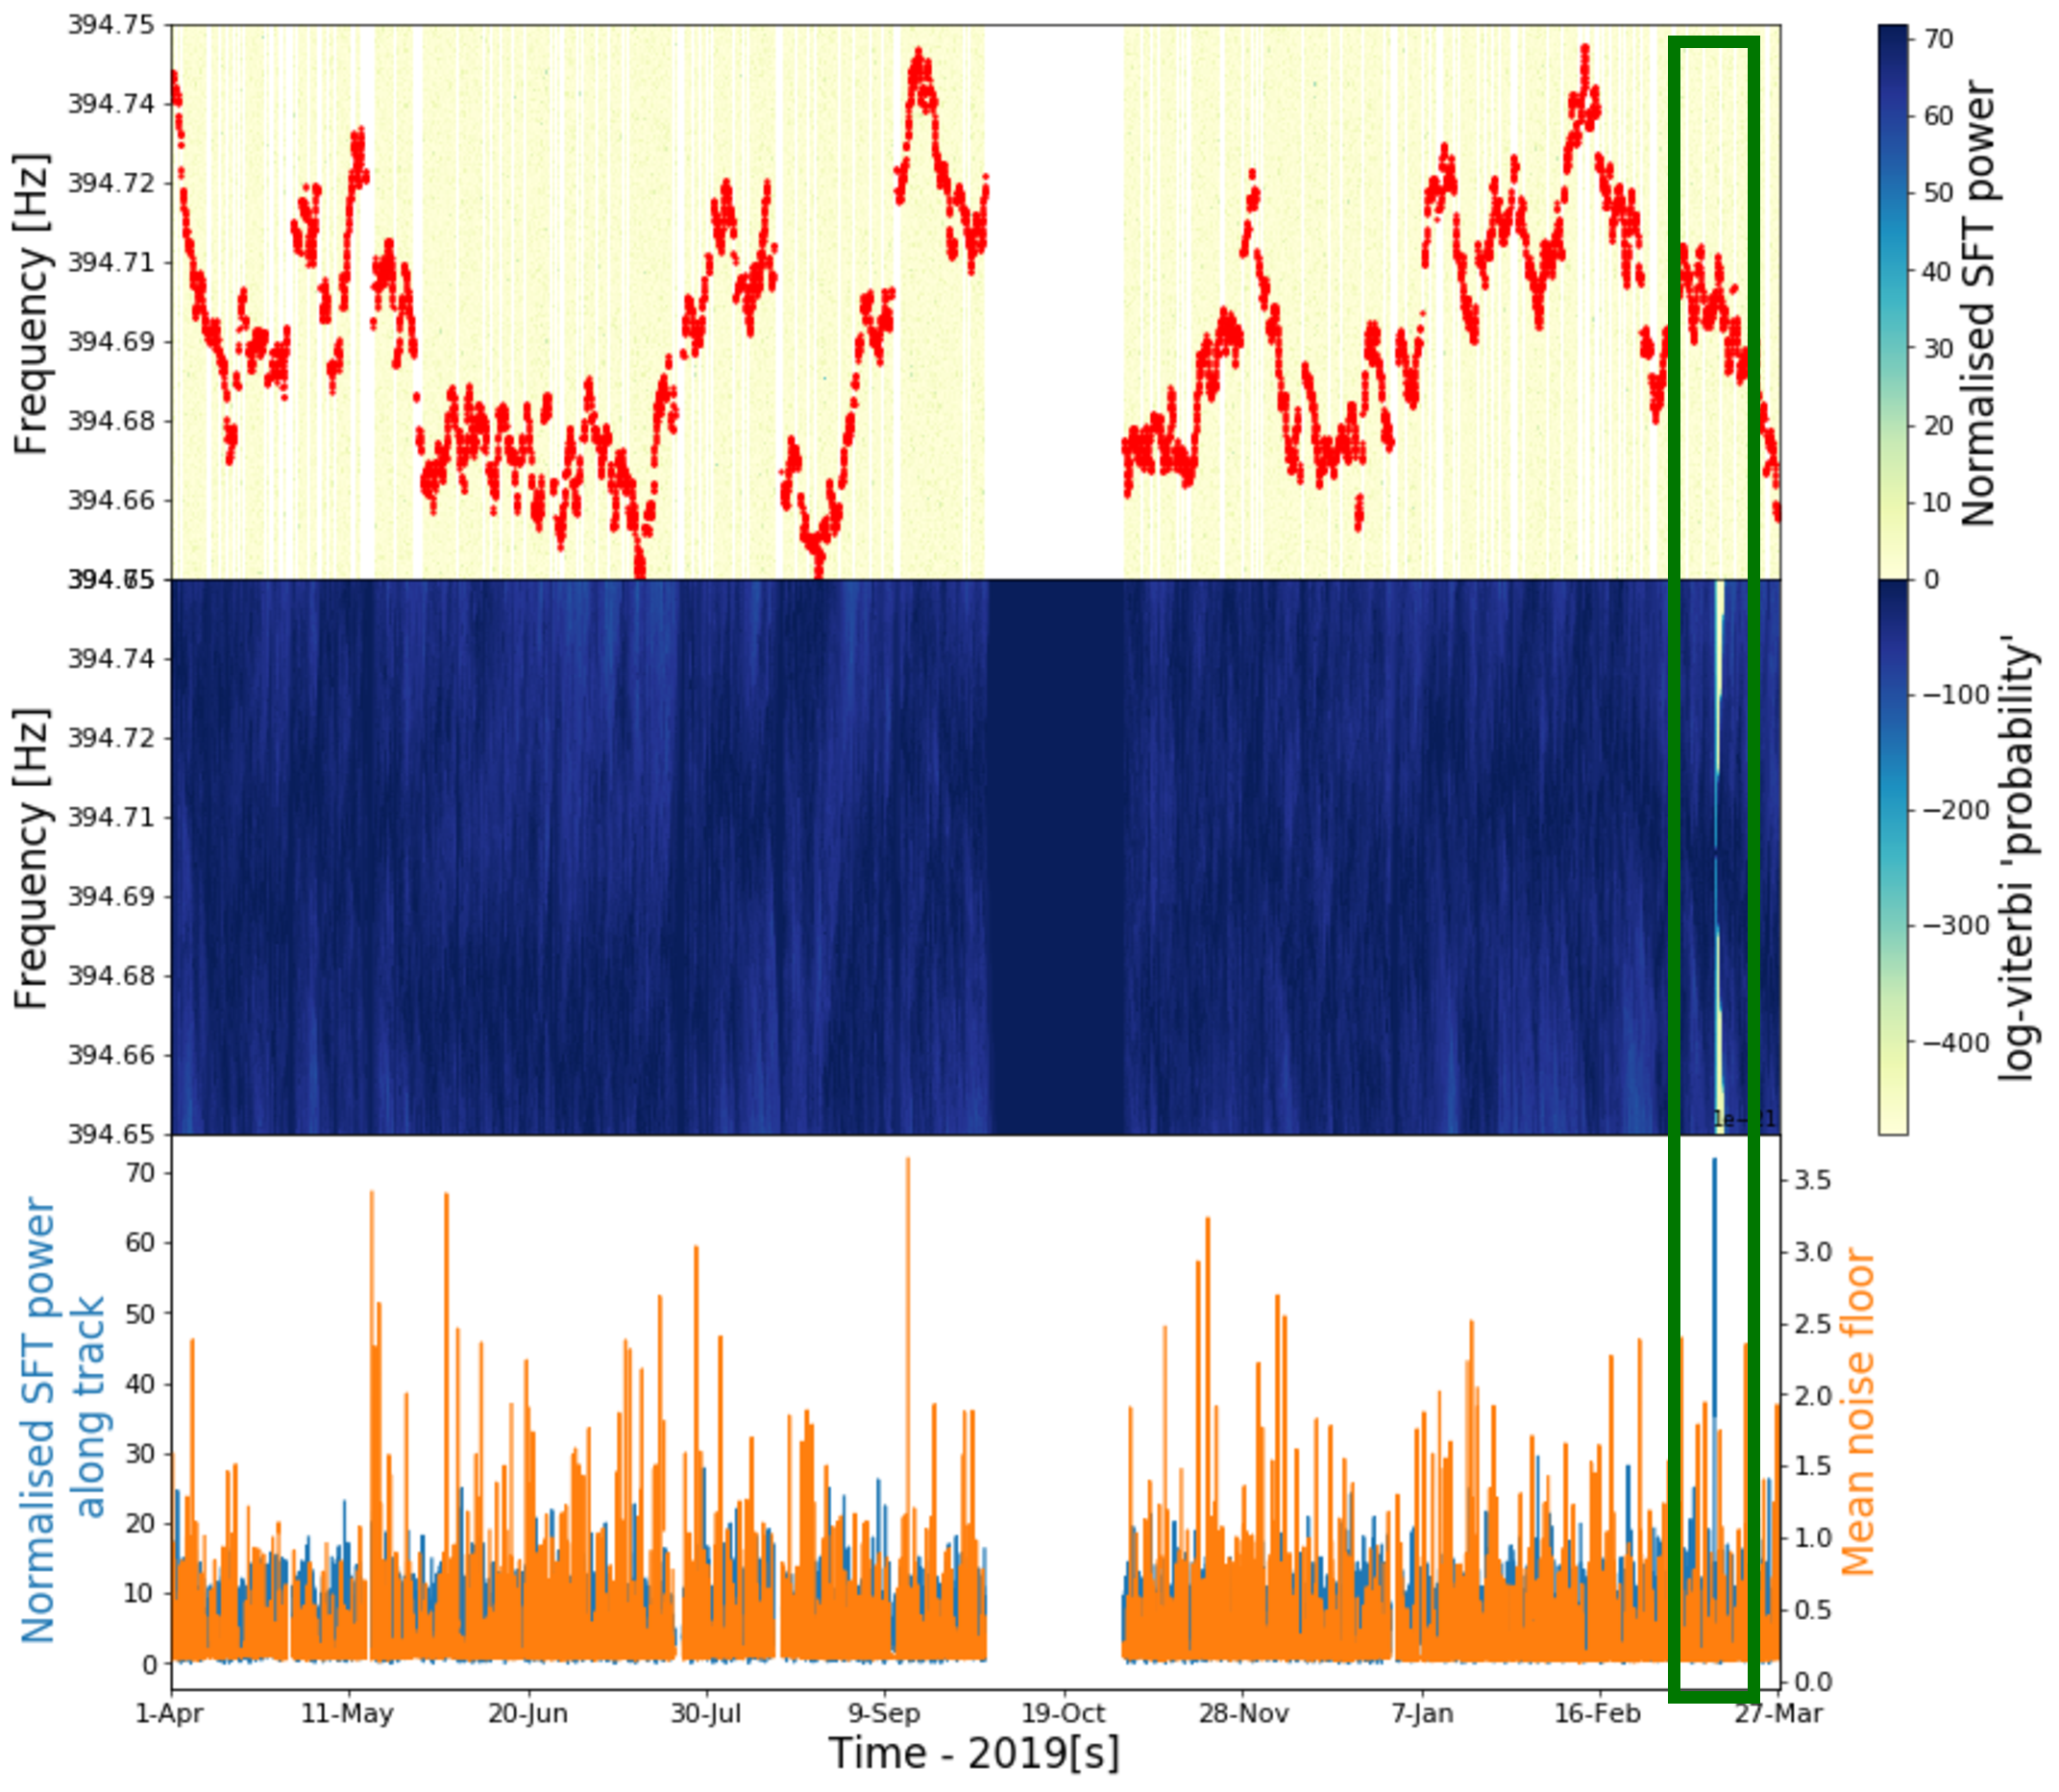
\includegraphics[width=\textwidth]{C6_detchar/linemixing/track_F394_65_394_75.pdf}
	\caption{\label{detchar:soap:calibrationlinemixing:4}}
\end{subfigure}
	\caption[Example of lines from ``calibration line mixing'' and ``calibration line non-linearity''.]{Example of lines from ``calibration line mixing'' and ``calibration line non-linearity''. Fig.~\ref{detchar:soap:calibrationlinemixing:3} and \ref{detchar:soap:calibrationlinemixing:4}  are examples of lines from ``calibration line mixing'', where these examples appear as short burst of \gls{SFT} power towards the end of the observing run. Fig.~\ref{detchar:soap:calibrationlinemixing:1} and \ref{detchar:soap:calibrationlinemixing:2} are examples of lines from `` calibration line non-linearity'', where these examples appear as short duration lines at the beginning of O3.  In each of these images I have highlighted the areas of interest with green squares. These are both short durations lines, therefore, SOAP will struggle to identify them in the Viterbi statistic if they do not have enough \gls{SFT} power, however is still visible in the Viterbi maps and Viterbi track.}
	\label{detchar:soap:calibrationlinemixing}
\end{figure}
%

Of the unknown line list, we 30\% of those on the \gls{LIGO} line list were in a sub-band which had a Viterbi statistic which crossed our detection threshold.  However, Viterbi statistics from sub-bands which contained these unknown lines and fell below the detection threshold showed signs in the Viterbi maps and Viterbi tracks which indicate an instrumental line is present. An example of this can be seen in Fig.~\ref{detchar:soap:unknown:1} where the in the second half of the observing run, the width of the Viterbi track narrows indicating that a narrow signal could be present. In the Viterbi maps and increase in the concentration of the log-probability around this frequency can be seen, again indicating a signal is present. Similar features can be see in Fig.~\ref{detchar:soap:unknown:2} and \ref{detchar:soap:unknown:3}.
For some other lines on \glspl{LIGO} unknown line list, such as in Fig.~\ref{detchar:soap:unknown:4}, there is no indication of an instrumental line in the SOAP outputs, however, in over 50\% of the undetected lines which have been investigated further, there is some evidence of a line in the other outputs of SOAP.
%
\begin{figure}[hpt]
	\centering
	\begin{subfigure}[h]{0.49\textwidth}
		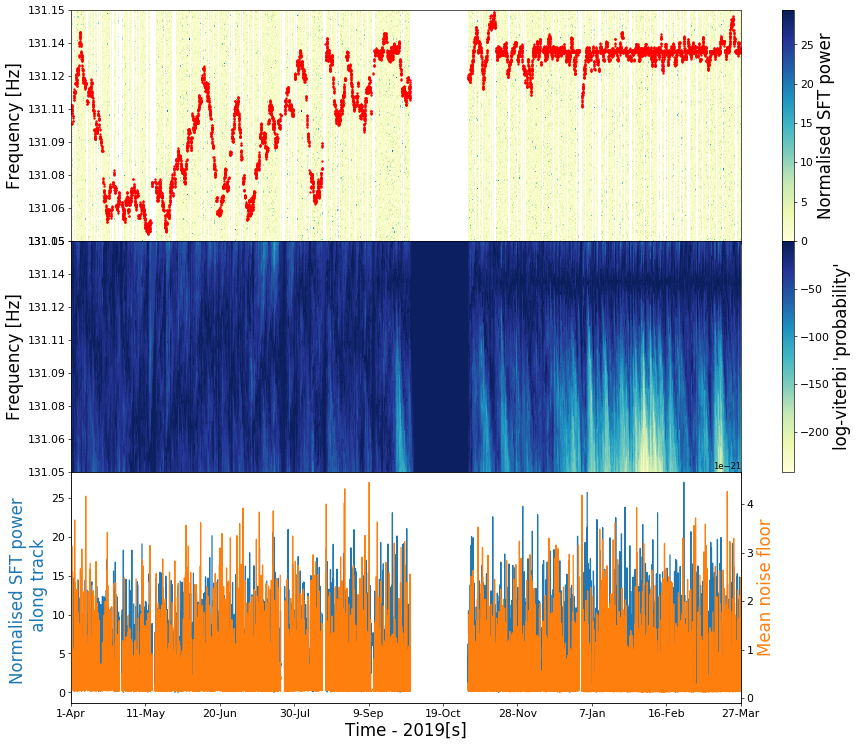
\includegraphics[width=\textwidth]{C6_detchar/track_F131_05_131_15.png}
		\caption{\label{detchar:soap:unknown:1}}
	\end{subfigure}
	\begin{subfigure}[h]{0.49\textwidth}
		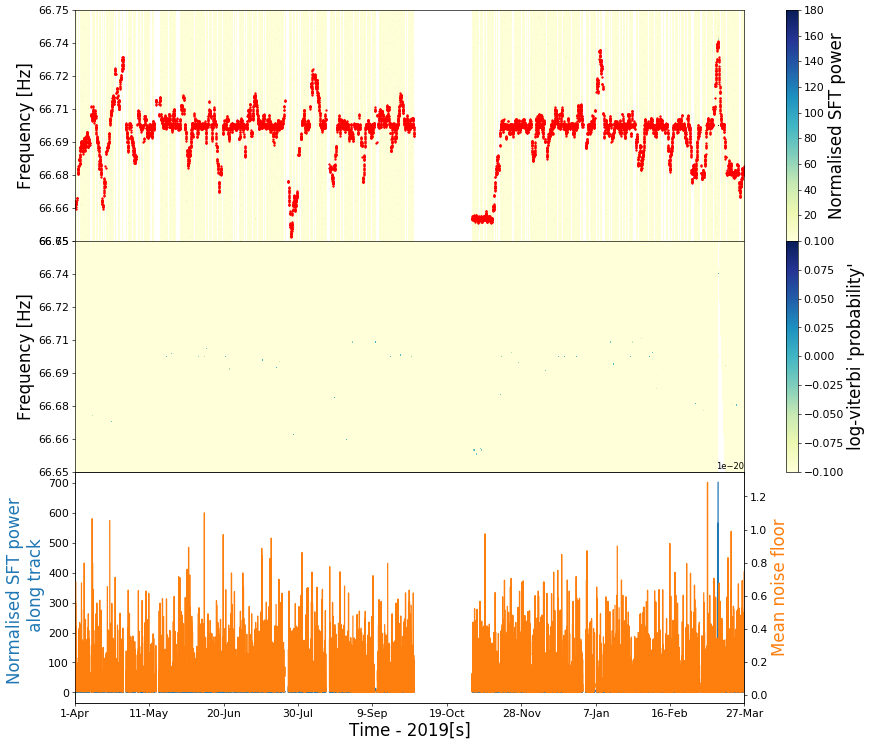
\includegraphics[width=\textwidth]{C6_detchar/track_F66_65_66_75.png}
		\caption{\label{detchar:soap:unknown:2}}
	\end{subfigure}
	
	\begin{subfigure}[h]{0.49\textwidth}
		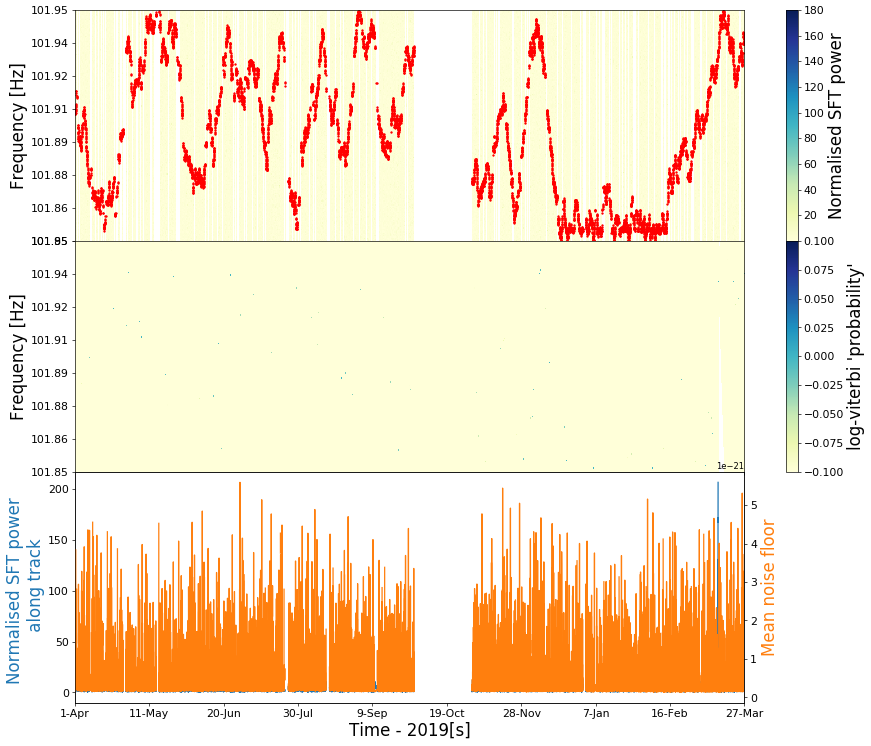
\includegraphics[width=\textwidth]{C6_detchar/track_F101_85_101_95.png}
		\caption{\label{detchar:soap:unknown:3}}
	\end{subfigure}
	\begin{subfigure}[h]{0.49\textwidth}
		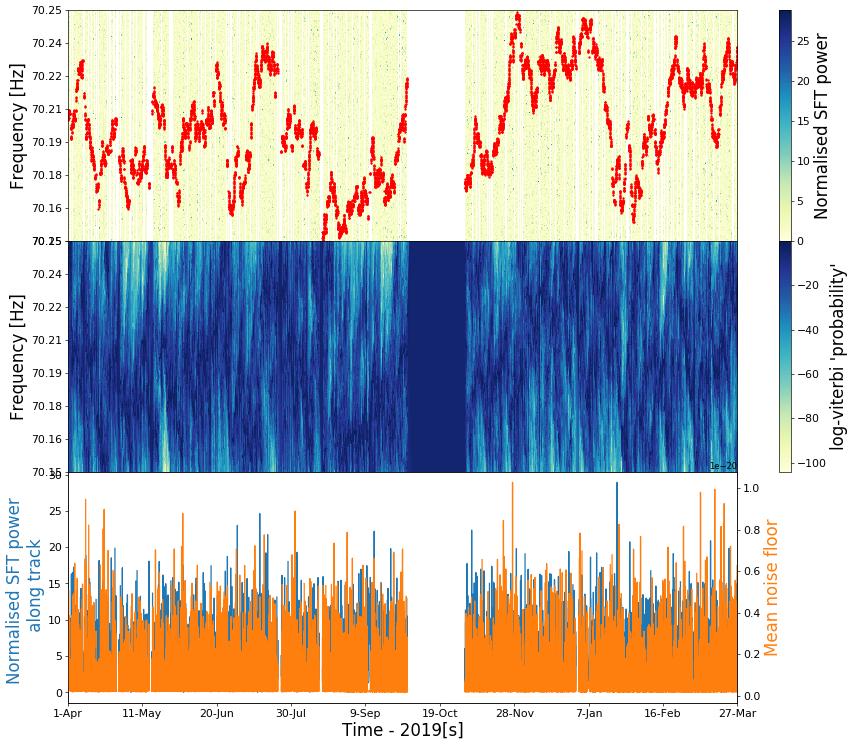
\includegraphics[width=\textwidth]{C6_detchar/track_F70_15_70_25.png}
		\caption{\label{detchar:soap:unknown:4}}
	\end{subfigure}
	\caption[lines from unknown sources]{Examples of unknown instrumental lines in H1 during the O3 run which were not identified by SOAP using the Viterbi statistic. These show the 1800s spectrograms for H1 in the top panel and the Viterbi maps in the second panel. The final panel shows the \gls{SFT} power along the Viterbi track and the mean noise floor in this band.  Fig.~\ref{detchar:soap:unknown:1}, \ref{detchar:soap:unknown:1} and \ref{detchar:soap:unknown:1} have areas of the Viterbi track which are narrow and are not spread over the entire band, indicating a non Gaussian signal is present. In Fig.\ref{detchar:soap:unknown:1} and \ref{detchar:soap:unknown:1} the Viterbi maps show some areas of high log-probability which are difficult to see at this resolution, hence the uniform appearance. }
	\label{detchar:soap:unknown}
\end{figure}
%

Therefore, one possible addition to the SOAP line search could be a method similar to that described in Chapter \ref{machine}, where here the Viterbi maps and Viterbi tracks associated with instrumental lines would be used as training data for a neural network. 
The neural networks could then be used to classify sub-bands into containing an instrumental line or Gaussian noise.
The difficulty with using these Viterbi maps as training examples is that we do have a set of training data with known labels. 
We could generate these labels from each sub-band in real data which contains an instrumental line, but this would require a large effort investigating the many sub-bands. Another method could be simulating instrumental lines, however this can be difficult due to the large variation in the types of instrumental line. Each of these types would need some functional representation such that they be generated, which would also need investigation in to the many types of line.
Methods such as in \citep{zevin2017GravitySpy} have had success using machine learning to classify short duration noise artefacts (glitches). This project uses time-frequency representations of the glitches that have been classified by volunteers from the public as training data for machine learning algorithms.
A similar approach could be used to classify the outputs of the SOAP search, where labels can be applied to sub-bands such that a machine learning algorithm can be trained.

Whilst SOAP did not identify all of the same lines as the methods in Sec.~\ref{detchar:monitor}, it did identify a large number of lines which did not appear in either the known of unknown line list.
For example, in Fig.~\ref{detchar:soap:newlines:1}, SOAP identified a line at $\sim 64.0$ Hz which does not currently appear in the \gls{LIGO} line list.
Further examples are at $\sim 299.7$ Hz in Fig.~\ref{detchar:soap:newlines:2} and $\sim 299.545$ Hz in Fig.~\ref{detchar:soap:newlines:3} which shows broader features of $\sim 0.005$ Hz wide. Finally Fig.~\ref{detchar:soap:newlines:4} shows that there may be multiple strong lines present within this sub-band, this is because the Viterbi track appears to have identified multiple features and `jumps' between these during the observing run.
In total, SOAP identified $\sim 200$ sub-bands which potentially contain an instrumental line which did not appear on the \gls{LIGO} line list. 
Whilst many of these will require further investigation, it demonstrates the ability of this search to identify new instrumental lines.

%
\begin{figure}[ht]
	\centering
	\begin{subfigure}[h]{0.49\textwidth}
		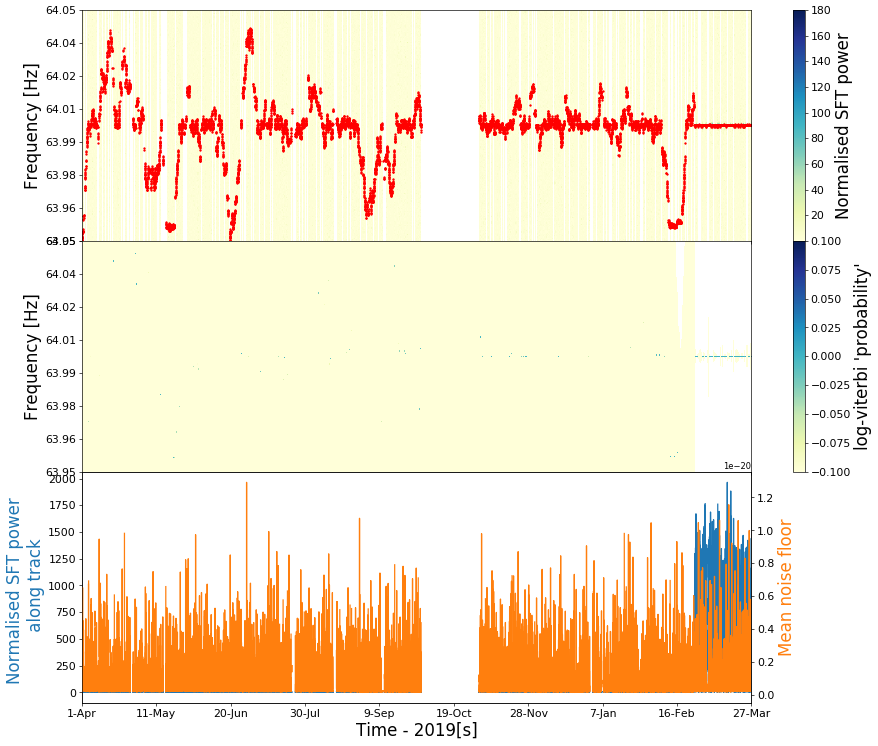
\includegraphics[width=\textwidth]{C6_detchar/track_F63_95_64_05.png}
		\caption{\label{detchar:soap:newlines:1}}
	\end{subfigure}
	\begin{subfigure}[h]{0.49\textwidth}
		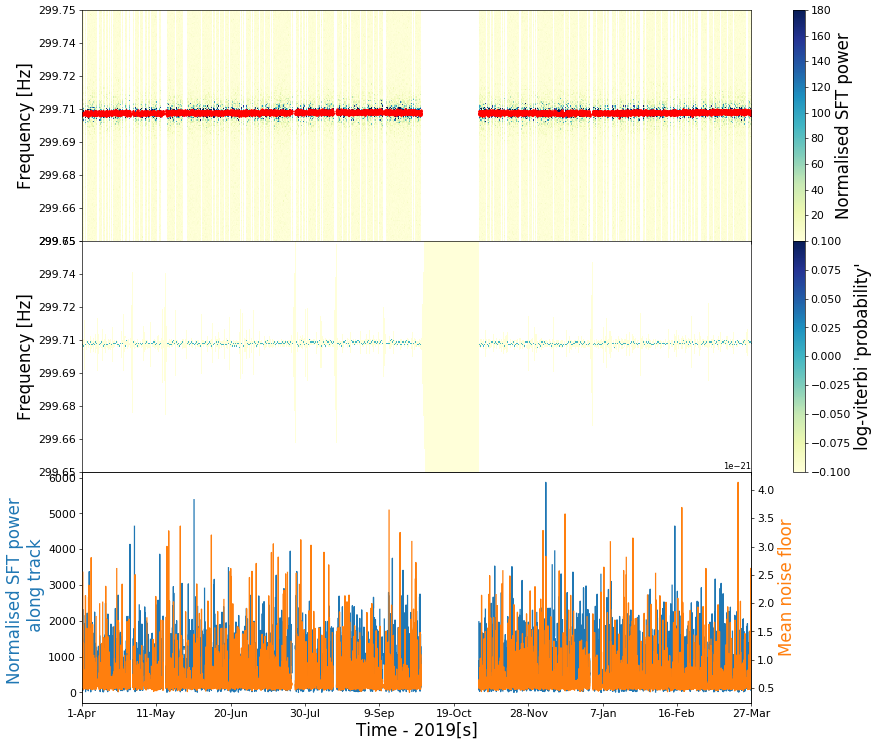
\includegraphics[width=\textwidth]{C6_detchar/track_F299_65_299_75.png}
		\caption{\label{detchar:soap:newlines:2}}
	\end{subfigure}
	
	\begin{subfigure}[h]{0.49\textwidth}
		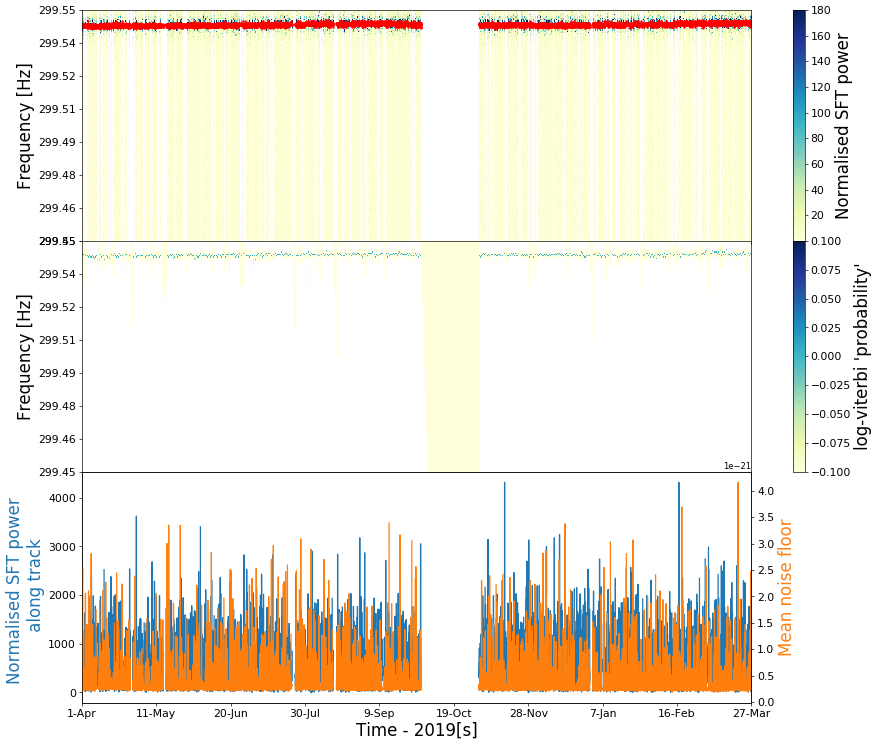
\includegraphics[width=\textwidth]{C6_detchar/track_F299_45_299_55.png}
		\caption{\label{detchar:soap:newlines:3}}
	\end{subfigure}
	\begin{subfigure}[h]{0.49\textwidth}
		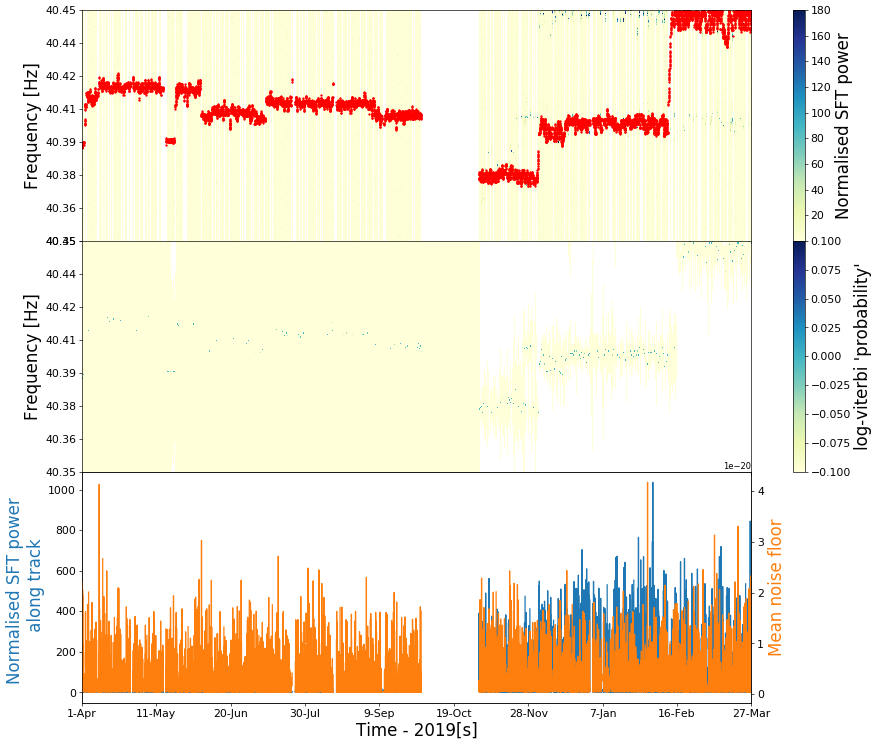
\includegraphics[width=\textwidth]{C6_detchar/track_F40_35_40_45.png}
		\caption{\label{detchar:soap:newlines:4}}
	\end{subfigure}
	\caption[New lines identified by SOAP.]{ Examples of instrumental lines identified by the SOAP line search in H1 during the O3 run which did not appear in \gls{LIGO} line lists are shown. Fig.~\ref{detchar:soap:newlines:2} and \ref{detchar:soap:newlines:3} show strong broad lines which do not wander in frequency. Fig.\ref{detchar:soap:newlines:1} shows a narrow band line which increases in \gls{SNR} in the final month of this O3. Finally Fig.~\ref{detchar:soap:newlines:4} shows multiple features within the sub band, where the Viterbi track `jumps' between the different features during the run.}
	\label{detchar:soap:newlines}
\end{figure}
%
\clearpage 

%%%%%%%%%%%
%%%%%%%%%%%%
\section{\label{detchar:summary}Summary pages}
%%%%%%%%%%%
%%%%%%%%%%%%%

Summary pages are an important tool when searching for both instrumental lines and astrophysical signals as there is a large amount of data in both frequency and time to search through, where for line searches there are also a large number of different channels. Summary pages
distil this data such that only the important information is shown. This
enables signals to be identified easily when looking through sub-bands. The
criteria when designing summary pages is that they are easy to navigate and the
important information is shown in a clear and concise way.  These summary pages exist
for the line searches in this chapter and the astrophysical searches from chapters \ref{soap} and \ref{machine} in \citep{bayleyHome} where this is only accessible by
\gls{LIGO}, Virgo and KAGRA members.
In this section I will explain the line summary pages, however, the astrophysical pages have a similar design.

Summary pages have currently been generated from the results of the SOAP search for observing runs O2 and O3 for
the two \gls{LIGO} detectors, where pages for other detectors and observing runs are planned. This was done for various timescales: for the
entire observing run and separately for each month.  This allows the variation
of a line to be observed for both the entire length of the run and shorter timescales. Once the detector, observing
run, and timescale is
set, we currently split the 40-500 Hz band into 0.1 Hz wide sub-bands.  
The SOAP search is then run on each sub-band using a flat transition matrix and the sum of \gls{SFT} powers along the Viterbi track as the detection 
statistic.
A flow diagram of how the SOAP search works for instrumental line searches can
be found in Fig.~\ref{detchar:summary:flow}.
%
%
\begin{figure}[hp]
	\centering
	

\tikzstyle{block} = [rectangle, draw, fill=blue!20, 
    text width=17em, text centered, rounded corners, minimum height=4em]
    
\tikzstyle{line} = [draw,line width=0.35mm, -latex']


\begin{tikzpicture}[node distance = 6em, auto]

    % Place node
    
  	\node [block] (sft) {1.\\ SFTs from Time series};
  
  	\node [block, below of=sft] (norm) {2. \\ Divide \gls{SFT} by running median and get power spectrum.};
  	\node [block, below of=norm] (narrow) {3. \\ Narrowband \gls{SFT} (0.2 Hz)};
	
	\node [block, below of=narrow] (soap) {4. \\ Run SOAP search and generate plots};
  
   \node [block, below of=soap] (summary) {5. \\ Generate summary page};

  
  % Draw edges
  \path [line] (sft) -- (norm);
  \path [line] (norm) -- (narrow);
  \path [line] (narrow) -- (soap);
  \path [line] (soap) -- (summary);
  

  
    
\end{tikzpicture}
	
	\caption[Flow diagram for SOAP line search.]{\label{detchar:summary:flow} The SOAP search for instrumental lines is simpler than other searches. A simple version of the search is run separately for each detector, where the raw \glspl{SFT} are divided by their running median, narrow-banded and then the search is run. }
	
\end{figure} 
These stages are as follows:
\begin{description}
	\item[1. \glspl{SFT} from time series] The \glspl{SFT} are generated for the \gls{GW} output channel. This is done by the Fscan search, therefore we do not repeat this process. Currently the search only runs on the \gls{GW} channel, however, in the future could be made to run on others.
	
	\item[2. Divide \gls{SFT} by running median] In this stage each
\gls{SFT} power spectrum is divided by its running median, where a correction factor is applied such that the data has a mean of 1. 
The running median has a window of width 100 bins, this was chosen such that broad features wide than this window are removed whilst outliers should remain. 
The output of this stage is then a high pass filtered \gls{SFT} power spectrum.
	
        \item[3. Narrow-band \gls{SFT}] The \gls{SFT} is then split into 0.1 Hz
wide sub-bands for the SOAP search to run on. These smaller bands are chosen as
the SOAP search only returns information on the most likely track in a sub-band, therefore, smaller
bands are not contaminated by areas of high power in neighbouring frequency
bands. 
	
        \item[4. Run SOAP and generate plots] This stage runs the SOAP search
with a flat transition matrix probability and generates plots as shown in
Fig.~\ref{detchar:soap:noiseplot}.
	
        \item[5. Generate summary page] Finally web pages known as `summary pages' are generated which summarise the SOAP outputs from each sub-band.
        This puts all sub-bands into a table where it can be ordered
by the value of the Viterbi statistic, or can be searched for particular
frequency bands.  Where selecting a frequency band will display the output plots shown throughout this chapter.
\end{description}

An example of a summary page is shown in Fig.~\ref{detchar:summary:plots}. This
has been annotated showing how to navigate the page.  There are generally two
separate parts to the page: selecting the observing run and frequencies, and
viewing the outputs.  The observing run is selected at the top of the page,
where currently this has been run on O2 and O3.  From this menu the
detector can be selected, currently \glspl{LIGO} H1 and L1 detectors are
present. On this page the desired frequency bands can be selected, where the output plots can be displayed. 
The key information of each page is the plots shown in
Figs.~\ref{detchar:soap:noiseplot} - \ref{detchar:soap:newlines}.
They show the time frequency spectrograms of the data, the output Viterbi tracks which
identify the most probable frequency track, the Viterbi maps which allow the
probability of a signal as a function of the time and frequency bin to be
viewed.  Finally they show the spectrogram power along the Viterbi track with
the mean noise floor of the detector during the observing run.  This should
provide useful information to asses whether an instrumental line in
present within a given sub-band.

To navigate each page, the left panel contains a calendar where the
start and end times of a result can be selected.  Currently there are
pre-defined times which can be selected from. This allows a line to be
investigated for a shorter or longer time period.  This can be useful when a
new instrumental line appears and it needs to be investigated only from when
the line appears.  Below this in the left panel of the page there is a table
where each cell is one of the sub-bands which was searched through. This allows
individual frequency bands of interest to be searched for as well as the table
to be limited between different frequencies.  The table contains four columns:
the frequency of the sub-bands, the Viterbi statistic, the $\sigma$ from the
mean of all the sub-band Viterbi statistics and extra information.  The first
two columns are self explanatory, the frequency range of the sub-band and the
resulting Viterbi statistic from that sub-band. The table can be ordered by the
Viterbi statistic such that only the highest values are investigated.  The
$\sigma$ from the mean is found by approximating the distribution of the
Viterbi statistics as a Gaussian.  A Gaussian is then fit to the distribution
using a simple least squares, each statistic then has a multiple of $\sigma$
away from the mean of this distribution.  This is an approximate calculation to
give a scale of how significant the statistic in that sub-band is.  The final
column contains any extra information which exists for that particular
frequency range.  For example, this is filled with other line list information
which has been collected from other search methods.  The loud features such as
Violin modes can then be marked. This means that these particular bands are
likely to have been investigated already allowing this search to focus on any
extra instrumental lines.
%
\begin{sidewaysfigure}[p]
	\centering
	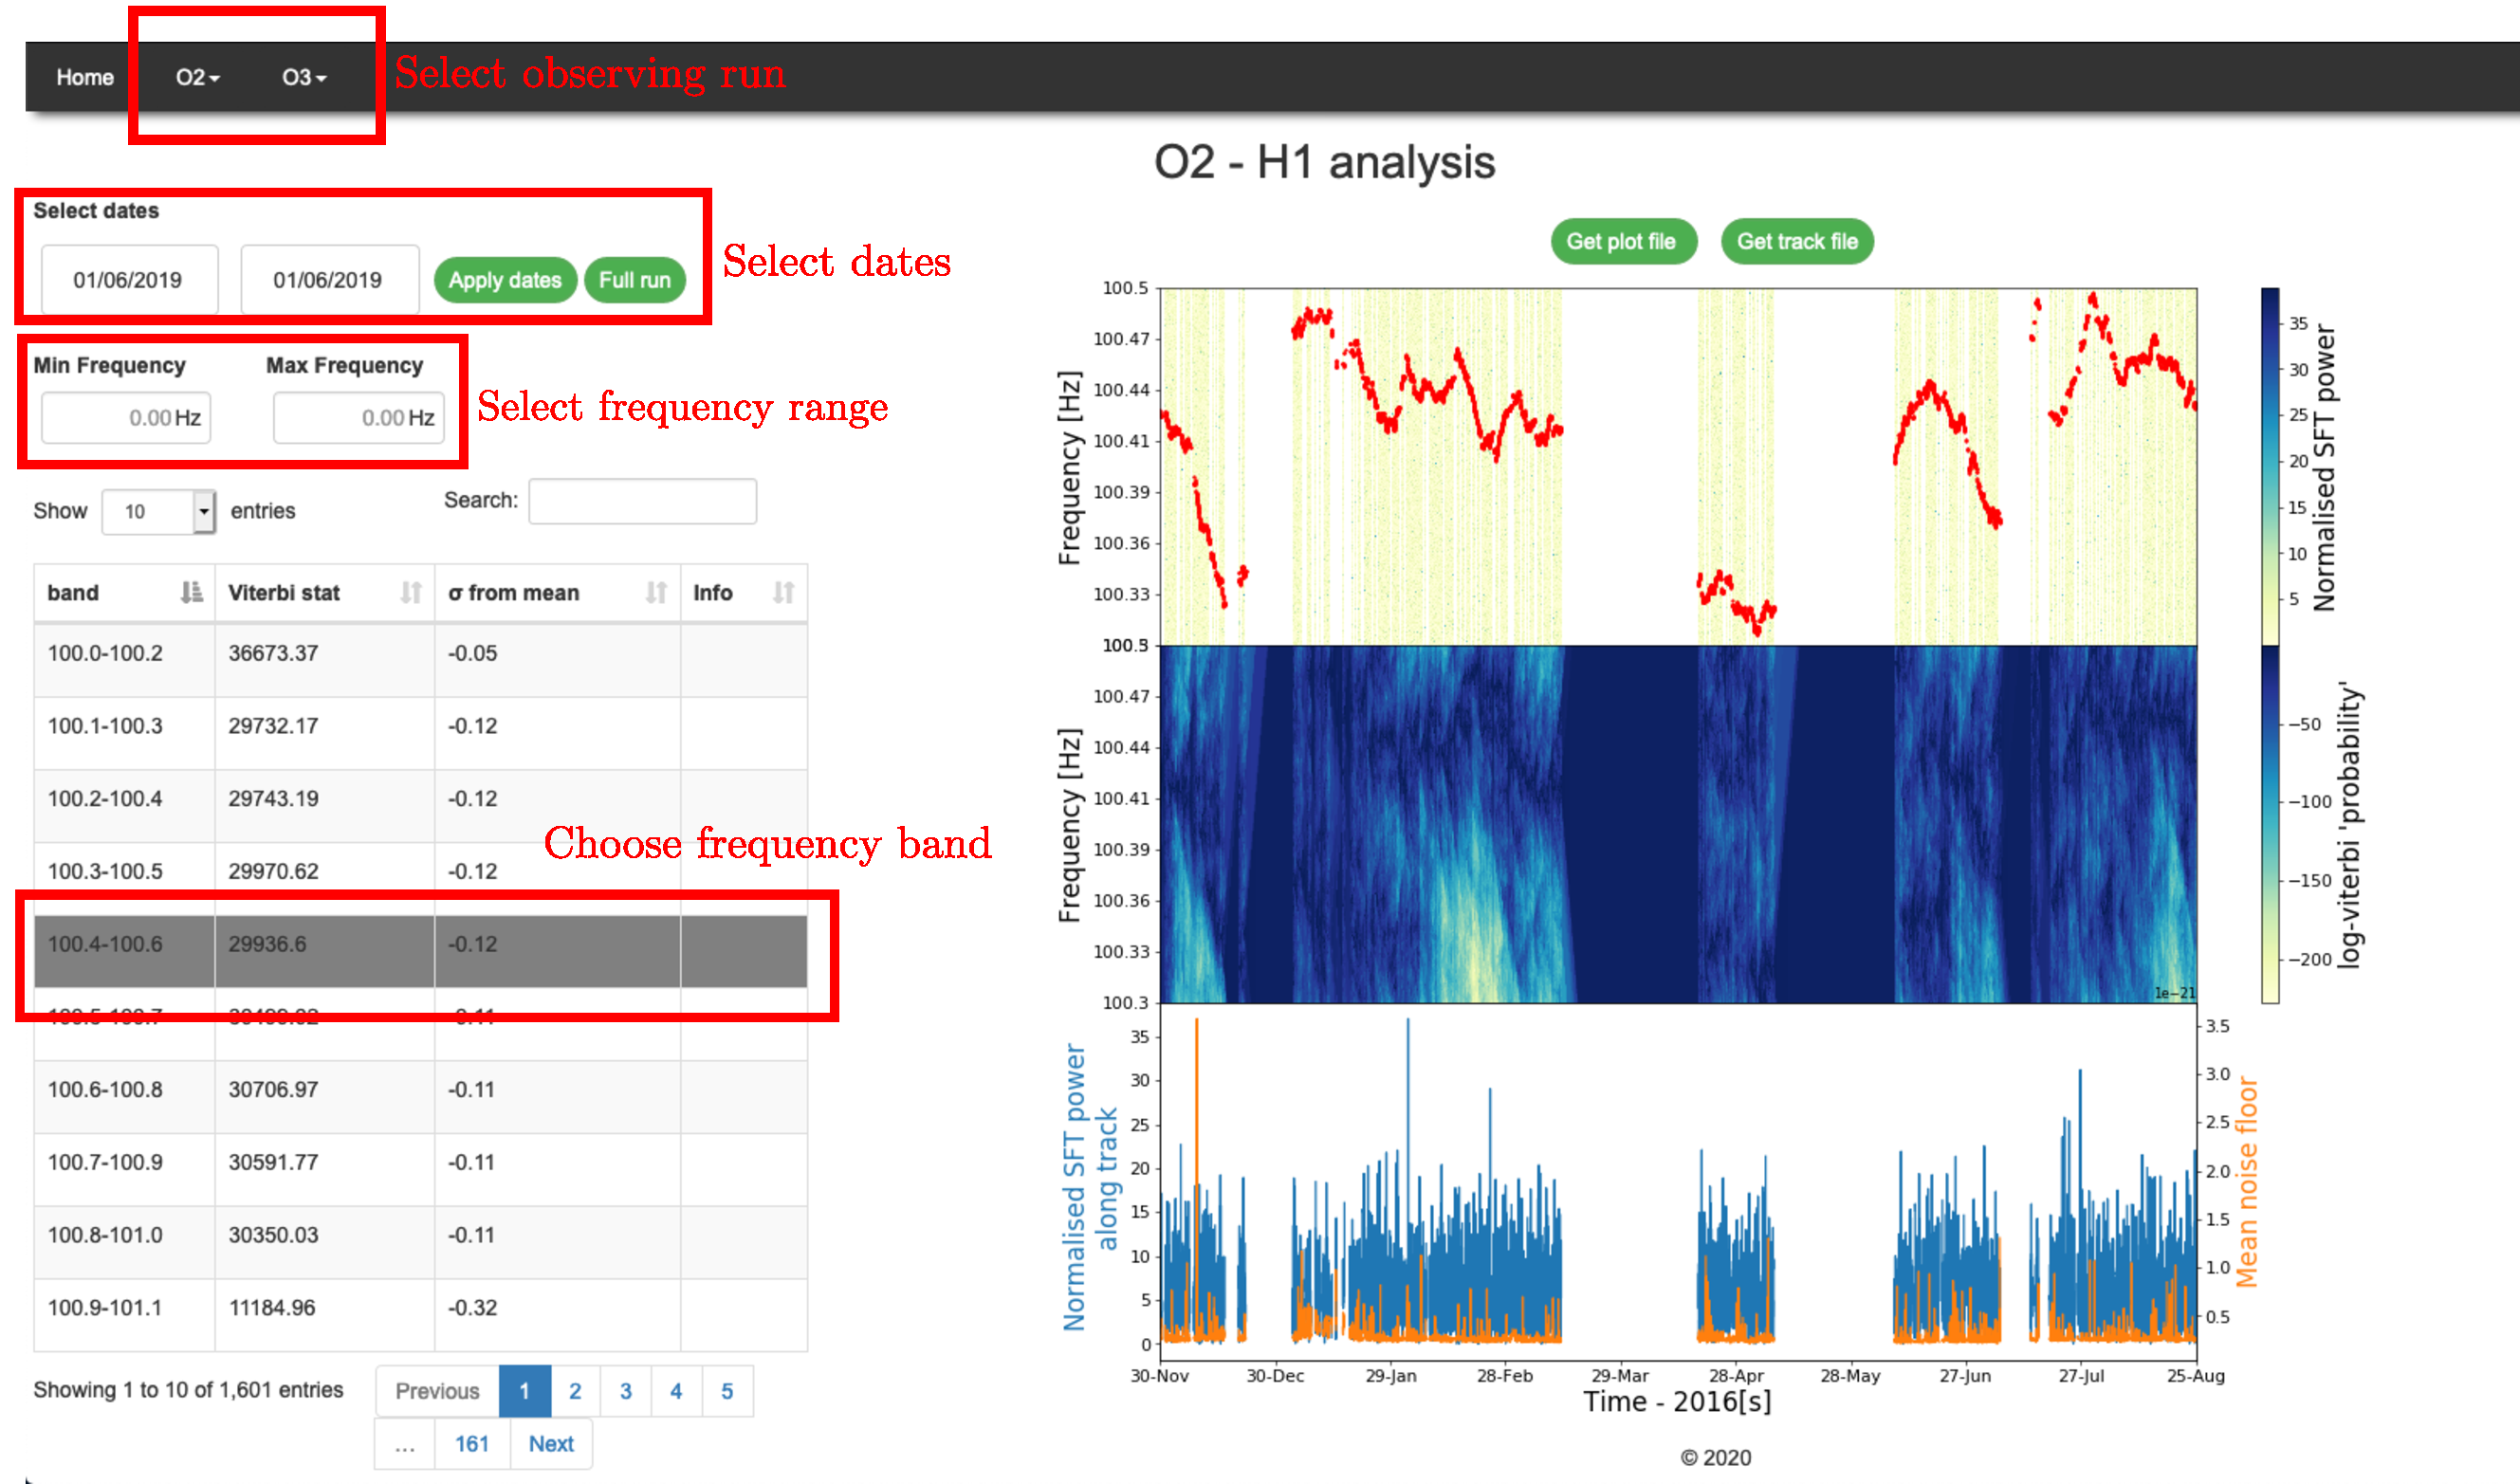
\includegraphics[width=\textwidth]{C6_detchar/summary_annot.pdf}
	\caption[Example summary page for SOAP search]{The summary pages are made for each observing run (in this case just O2 and O3). The range of times can then be selected from a set of start and end times. This is in general the entire observing run and monthly runs of this search. These pages can be found at \citep{bayleyHome}}
	\label{detchar:summary:plots}
\end{sidewaysfigure}
%

The summary pages offer a way to easily view the outputs of the SOAP line search, where sub-bands which are identified by SOAP as containing a potential signal can be investigated further. 
The aim of this tool is to be used alongside existing methods described in Sec.~\ref{detchar:monitor} to aid in the identification of potential instrumental lines.
\joe{just a little more}


